%% This is the ctufit-thesis example file. It is used to produce theses
%% for submission to Czech Technical University, Faculty of Information Technology.
%%
%% Get the newest version from
%% https://gitlab.fit.cvut.cz/theses-templates/FITthesis-LaTeX
%%
%%
%% Copyright 2021, Eliska Sestakova and Ondrej Guth
%%
%% This work may be distributed and/or modified under the
%% conditions of the LaTeX Project Public Licenese, either version 1.3
%% of this license or (at your option) any later version.
%% The latest version of this license is in
%%  https://www.latex-project.org/lppl.txt
%% and version 1.3 or later is part of all distributions of LaTeX
%% version 2005/12/01 or later.
%%
%% This work has the LPPL maintenance status `maintained'.
%%
%% The current maintainer of this work is Ondrej Guth.
%% Contact ondrej.guth@fit.cvut.cz for bug reports.
%% Alternatively, submit bug reports into the tracker at
%% https://gitlab.fit.cvut.cz/theses-templates/FITthesis-LaTeX/issues
%%
%%

%%%%%%%%%%%%%%%%%%%%%%%%%%%%%%%%%%%%%%%%%
% CLASS OPTIONS
% language: czech/english/slovak
% thesis type: bachelor/master/dissertation
%%%%%%%%%%%%%%%%%%%%%%%%%%%%%%%%%%%%%%%%%
\documentclass[english,bachelor,unicode]{ctufit-thesis}

%%%%%%%%%%%%%%%%%%%%%%%%%%%%%%%%%%
% FILL IN THIS INFORMATION
%%%%%%%%%%%%%%%%%%%%%%%%%%%%%%%%%%
\ctufittitle{Generating music using neural networks} % replace with the title of your thesis
\ctufitauthorfull{Jan Šimerda} % replace with your full name (first name(s) and then family name(s) / surname(s)) including academic degrees
\ctufitauthorsurnames{Šimerda} % replace with your surname(s) / family name(s)
\ctufitauthorgivennames{Jan} % replace with your first name(s) / given name(s)
\ctufitsupervisor{Mgr.\,Jan Tyl} % replace with name of your supervisor/advisor (include academic degrees)
\ctufitdepartment{Department of Applied Mathematics} % replace with the department of your defence
\ctufityear{2022} % replace with the year of your defence
\ctufitdeclarationplace{Prague} % replace with the place where you sign the declaration
\ctufitdeclarationdate{\today} % replace with the date of signature of the declaration
\ctufitabstractCZE{
    Tato bakalářská práce zkoumá využití umělých neuronových sítí v oblasti strojového generování hudby.
    Zaměřili jsme se na využití technik používaných ve zpracování přirozeného jazyka založených na attention mechanismu.
    Práce popisuje celý proces generování hudby od výběru dat, přes \textit{tokenizaci} (transformace hudby ze surových dat do formátu vhodného pro vybrané modely) až po trénování modelu.

    % TODO: review, whether LSTM architecture should be kept
    Použili jsme nejmodernější modely založené na \textit{Transformer} a \textit{LSTM} architekturách, běžně užívaných v NLP, abychom získali odpověď na otázku, jestli lze tyto modely, které mají skvělé výsledky v doménách generování textu a strojového překladu, použít také pro generování hudby.
    Vyzkoušeli jsme také několik navrhovaných vylepšení Transformer modelu a attention mechanismu a porovnali je s původním Transformer modelem.

    Pro trénování neuronových sítí jsme využili datasety MAESTRO a GiantMIDI, které obsahují stovky hodin klasických klavírních skladeb.
    Skladby použité pro trénování modelů jsou v symbolické MIDI reprezentaci.

    Zjistili jsme, že \ldots % TODO: sum up achieved results
}
\ctufitabstractENG{
    This thesis aims at using artificial neural networks in machine music generation.
    We emphasized using natural language processing techniques based on attention mechanisms.
    The work describes the whole music generation pipeline from data selection through \textit{tokenization} (transforming music from raw data into a format digestible by selected models) up to model training.

    % TODO: review, whether LSTM architecture should be kept
    We used state-of-the-art models based on the \textit{Transformer} and the \textit{LSTM} architectures commonly used in NLP to answer whether these well-performing models in domains like text generation or text translation can also be used to generate music.
    We also tested some proposed enhancements to the Transformer model and the attention mechanism and compared them to the vanilla Transformer model.

    We used the MAESTRO and the GiantMIDI datasets for the training process that contain hundreds of hours of classical piano pieces.
    The songs used for training the models are in symbolic MIDI representation.

    We found out that \ldots % TODO: sum up achieved results
}
\ctufitkeywordsCZE{generování hudby, MIDI, transformers, zpracování přirozeného jazyka, umělé neuronové sítě, Tensorflow, Python}
\ctufitkeywordsENG{music generation, MIDI, transformers, natural language processing, artificial neural networks, Tensorflow, Python}
%%%%%%%%%%%%%%%%%%%%%%%%%%%%%%%%%%
% END FILL IN
%%%%%%%%%%%%%%%%%%%%%%%%%%%%%%%%%%

%%%%%%%%%%%%%%%%%%%%%%%%%%%%%%%%%%
% CUSTOMIZATION of this template
% Skip this part or alter it if you know what you are doing.
%%%%%%%%%%%%%%%%%%%%%%%%%%%%%%%%%%

\RequirePackage{iftex}[2020/03/06]
\iftutex % XeLaTeX and LuaLaTeX
\RequirePackage{ellipsis}[2020/05/22] %ellipsis workaround for XeLaTeX
\else
\RequirePackage[utf8]{inputenc}[2018/08/11] %this file encoding
\RequirePackage{lmodern}[2009/10/30] % vector flavor of Computer Modern font
\fi

% hyperlinks
\RequirePackage[pdfpagelayout=TwoPageRight,colorlinks=false,allcolors=decoration,pdfborder={0 0 0.1}]{hyperref}[2020-05-15]

% uncomment the following to hide all hyperlinks
% \RequirePackage[pdfpagelayout=TwoPageRight,hidelinks]{hyperref}[2020-05-15]

\RequirePackage{pdfpages}[2020/01/28]

\setcounter{secnumdepth}{4} % numbering sections; 4: subsubsection


%%%%%%%%%%%%%%%%%%%%%%%%%%%%%%%%%%
% CUSTOMIZATION of this template END
%%%%%%%%%%%%%%%%%%%%%%%%%%%%%%%%%%


%%%%%%%%%%%%%%%%%%%%%%
% DEMO CONTENTS SETTINGS
% You may choose to modify this part.
%%%%%%%%%%%%%%%%%%%%%%
\usepackage{dirtree}
\usepackage{lipsum,tikz}
\usepackage{csquotes}
\usepackage[style=iso-numeric]{biblatex}
\addbibresource{text/bib-database.bib}
\usepackage{listings} % typesetting of sources
% \usepackage{minted} % typesetting of sources
\usepackage{musicography} % musical symbols
\usepackage{blkarray}
\usepackage{amsmath} % matrices

%theorems, definitions, etc.
\theoremstyle{plain}
\newtheorem{theorem}{Věta}
\newtheorem{lemma}[theorem]{Tvrzení}
\newtheorem{corollary}[theorem]{Důsledek}
\newtheorem{proposition}[theorem]{Návrh}
\newtheorem{definition}[theorem]{Definice}
\theoremstyle{definition}
\newtheorem{example}[theorem]{Příklad}
\theoremstyle{remark}
\newtheorem{note}[theorem]{Poznámka}
\newtheorem*{note*}{Poznámka}
\newtheorem{remark}[theorem]{Pozorování}
\newtheorem*{remark*}{Pozorování}
\numberwithin{theorem}{chapter}
%theorems, definitions, etc. END
%%%%%%%%%%%%%%%%%%%%%%
% DEMO CONTENTS SETTINGS END
%%%%%%%%%%%%%%%%%%%%%%

\begin{document}
    \frontmatter\frontmatterinit % do not remove these two commands

    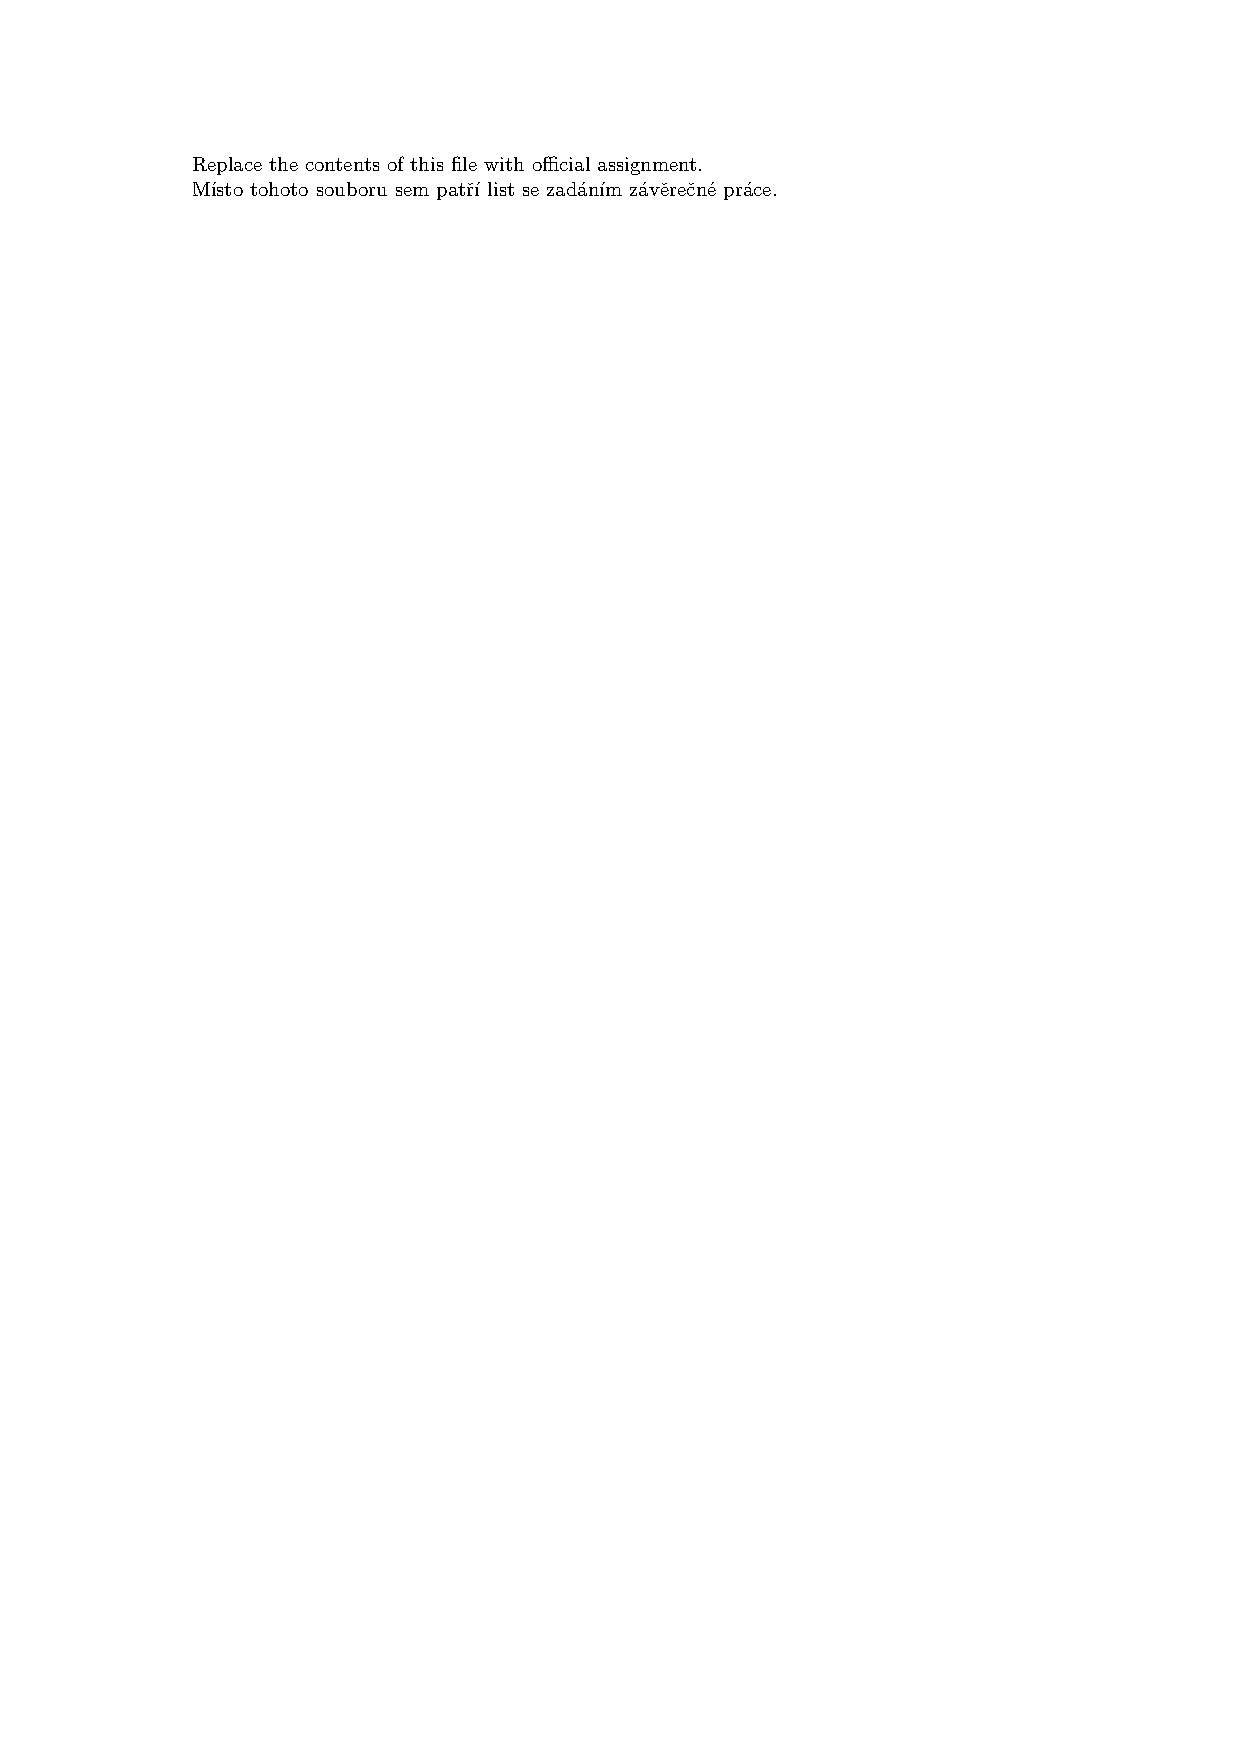
\includepdf{assets/assignment.pdf} % replace that file with your thesis assignment provided by study office

    \thispagestyle{empty}\cleardoublepage\maketitle % do not remove these three commands

    \imprintpage % do not remove this command

    \tableofcontents % do not remove this command
%%%%%%%%%%%%%%%%%%%%%%
% list of other contents: figures, tables, code listings, algorithms, etc.
% add/remove commands accordingly
%%%%%%%%%%%%%%%%%%%%%%
    \listoffigures % list of figures
%%%%%%%%%%%%%%%%%%%%%%
% list of other contents END
%%%%%%%%%%%%%%%%%%%%%%

%%%%%%%%%%%%%%%%%%%
% ACKNOWLEDGMENT
% FILL IN / MODIFY
% This is a place to thank people for helping you. It is common to thank your supervisor.
%%%%%%%%%%%%%%%%%%%
    \begin{acknowledgmentpage}
        I would like to thank \ldots % TODO: write acknowledgement
    \end{acknowledgmentpage}
%%%%%%%%%%%%%%%%%%%
% ACKNOWLEDGMENT END
%%%%%%%%%%%%%%%%%%%


%%%%%%%%%%%%%%%%%%%
% DECLARATION
% FILL IN / MODIFY
%%%%%%%%%%%%%%%%%%%
% INSTRUCTIONS
% ENG: choose one of approved texts of the declaration. DO NOT CREATE YOUR OWN. Find the approved texts at https://courses.fit.cvut.cz/SFE/download/index.html#_documents (document Declaration for FT in English)
% CZE/SLO: Vyberte jedno z fakultou schvalenych prohlaseni. NEVKLADEJTE VLASTNI TEXT. Schvalena prohlaseni najdete zde: https://courses.fit.cvut.cz/SZZ/dokumenty/index.html#_dokumenty (prohlášení do ZP)
    \begin{declarationpage}
        I hereby declare that the presented thesis is my own work and that I have cited all
        sources of information in accordance with the Guideline for adhering to ethical
        principles when elaborating an academic final thesis.\\
        I acknowledge that my thesis is subject to the rights and obligations stipulated by the
        Act No. 121/2000 Coll., the Copyright Act, as amended, in particular that the Czech
        Technical University in Prague has the right to conclude a license agreement on the
        utilization of this thesis as a school work under the provisions of Article 60 (1) of the
        Act
    \end{declarationpage}
%%%%%%%%%%%%%%%%%%%
% DECLARATION END
%%%%%%%%%%%%%%%%%%%

    \printabstractpage % do not remove this command

%%%%%%%%%%%%%%%%%%%
% SUMMARY
% FILL IN / MODIFY
% OR REMOVE ENTIRELY (upon agreement with your supervisor)
% (appropriate to remove in most theses)
%%%%%%%%%%%%%%%%%%%
%    \begin{summarypage}
%        \section*{Summary section}
%
%        \lipsum[1][1-8]
%
%        \section*{Summary section}
%
%        \lipsum[2][1-6]
%
%        \section*{Summary section}
%
%        \lipsum[3]
%
%        \section*{Summary section}
%
%        \lipsum[2]
%
%        \section*{Summary section}
%
%        \lipsum[1][1-8] Lorem lorem lorem.
%    \end{summarypage}
%%%%%%%%%%%%%%%%%%%
% SUMMARY END
%%%%%%%%%%%%%%%%%%%

%%%%%%%%%%%%%%%%%%%
% ABBREVIATIONS
% FILL IN / MODIFY
% OR REMOVE ENTIRELY
% List the abbreviations in lexicography order.
%%%%%%%%%%%%%%%%%%%


    \chapter{Lists of abbreviations}\label{ch:lists-of-abbreviations}

    \begin{tabular}{rl}
        AI      & Artificial Intelligence                                       \\
        ANN     & Artificial Neural Network                                     \\
        GAN     & Generative Adversarial Networks                               \\
        GPU     & Graphics Processing Unit                                      \\
        GRU     & Gated Recurrent Unit                                          \\
        LSTM    & Long Short-Term Memory                                        \\
        MAESTRO & MIDI and Audio Edited for Synchronous TRacks and Organization \\
        MIDI    & Musical Instrument Digital Interface                          \\
        NLP     & Natural Language Processing                                   \\
        RNN     & Recurrent Neural Network
    \end{tabular}
%%%%%%%%%%%%%%%%%%%ß
% ABBREVIATIONS END
%%%%%%%%%%%%%%%%%%%

    \mainmatter\mainmatterinit % do not remove these two commands

%%%%%%%%%%%%%%%%%%%
% THE THESIS
% MODIFY ANYTHING BELOW THIS LINE
%%%%%%%%%%%%%%%%%%%

    % Introduction
%---------------------------------------------------------------
\chapter*{Introduction}\label{ch:introduction}
\addcontentsline{toc}{chapter}{Introduction}
\markboth{Introduction}{Introduction}
%---------------------------------------------------------------
\setcounter{page}{1}

From the beginnings of modern humanity to this day and age, music has played an ever-present part in our lives.
Up until the upswing of the computer era, music composing was carried out mainly by humans, though there were some experiments with algorithmic music generation even before the first computer\footnote{the musical piece was composed using defined musical segments selected by dice roll~\cite{music-generation-history}}.
However, after scientists developed the first computers, people became interested in whether computers could also perform complex and creative tasks like self-driving or music generation.

Lately, \textit{artificial} intelligence has crept into our lives more than ever before.
From fraud detection, personalization, and content recommendation to image enhancement and facial recognition, AI helped drive all those things forward.
The inventions in artificial intelligence and machine learning techniques, along with advances in computer hardware performance, helped tremendously with the ability to perform complex tasks like those mentioned above.

Even music did not escape this evolution, and there have been attempts at using \textit{RNN}s, \textit{GRU}s, and \textit{LSTM}s for automated music generation with promising results.
With the \textit{Transformer} being one of the newer models, not many papers exist on utilizing it for music composition, in contrast to recurrent neural networks.

This thesis aims to research possible ways of generating musical compositions using \textit{artificial neural networks}.
Specifically, this work focuses on leveraging neural network architectures used in \textit{natural language processing} (GRU, LSTM, Transformer, \ldots).
The goal of the practical part of this work is to create a functioning music generation model that would be able to generate songs from scratch or generate continuation for an existing song.
This solution could help music composers with the creative part of music composition.

% Music theory
%---------------------------------------------------------------


\addcontentsline{toc}{chapter}{Music theory}
\markboth{Music theory}{Music theory}

\begin{chapterabstract}
    Since our goal is to research music and see how we can compose it algorithmically, it is reasonable to start with some fundamentals of music theory.
    This chapter will cover the basics of sound, music, and different music terminology.
    % TODO: maybe add some more lines
\end{chapterabstract}


\section{Sound}\label{sec:sound}

We can define \textit{sound} as an auditory sensation we perceive when exposed to certain types of atmospheric disturbances (sound waves).
Sound waves are produced by a vibration of some source, like human vocal cords, an instrument, or a loudspeaker.~\cite{sound}


\section{Music}\label{sec:music}

\textit{Music} can be defined as ``organized sound'' in the broadest possible sense.
This open-ended and safe definition is coherent regardless of era, style, culture, or the mechanics of musical organization.
Each successive historical era produces musically artistic expressions of its own time and musical aura.
The study of \textit{Music Theory} is how we investigate this.~\cite{music-theory-andrew}


\section{Music theory}\label{sec:music-theory}

As described by~\cite{music-theory-andrew}, Music Theory is a scientific study of music and its organizational characteristics.
Its purpose is to examine questions like how we perceive music aurally, how we experience music aesthetically, and how we can symbolize it visually.
We can learn to associate sounds with symbols to aid our ability to perceive music at levels of increasing depth and better our comprehension.

Moreover,~\cite{music-theory-andrew} states that while studying music, we employ two approaches:
\begin{itemize}
    \item \textit{Analysis} -- we learn to employ commonly accepted techniques and specialized language to describe the musical organization.
    These techniques share analytical language throughout the community of musicians.
    \textit{This is conceptual knowledge and evaluation.}
    \item \textit{Composition} -- either by actively creating our own works or (as is the case of this thesis) imitating or emulating the works of earlier composers.
    \textit{This is active knowledge and procedure.}
\end{itemize}


\section{Pitch}\label{sec:pitch}

We can describe \textit{pitch} as a perceived highness or lowness of a sound;
this directly corresponds to the frequency of the sensed sound.
On a piano, there are 88 \textit{notes}.
Each of the notes corresponds to a different pitch.
Notes placed on the left side of a piano correspond to a lower pitch, and as we go to the right side of the piano, the pitch gets progressively higher~\ref{fig:piano}.~\cite{music-theory}

\begin{figure}
    \centering
    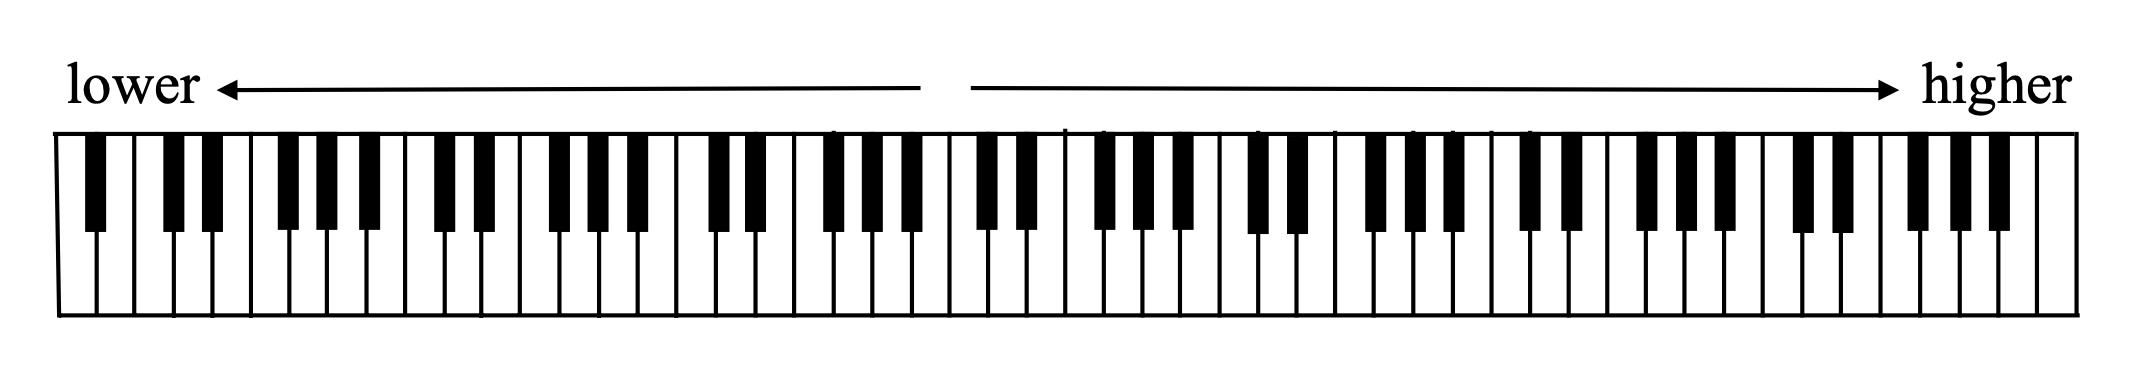
\includegraphics[width=\textwidth]{assets/piano}
    \caption{~A piano with 88 keys and indicated pitches~\cite{music-theory}}\label{fig:piano}
\end{figure}


\section{Notation}\label{sec:notation}

Notes are written on a five-line \textit{staff} (figure~\ref{fig:staff}).
A \textit{clef} orients the lines to a reference point.
For example, when placed on a five-line staff, the \textit{G clef} becomes the \textit{treble clef}, the most well-known \textit{clef}.
In treble clef, the notes on the lines are E--G--B--D--F from lowest to highest, often remembered through the traditional mnemonic\footnote{Every Good Boy Does Fine}.
The spaces are F--A--C--E from lowest to highest.
\textit{Staves} (the plural of ``staff'') are extended by the ledger lines (figure~\ref{fig:staff}).~\cite{music-theory}


\begin{figure}
    \centering
    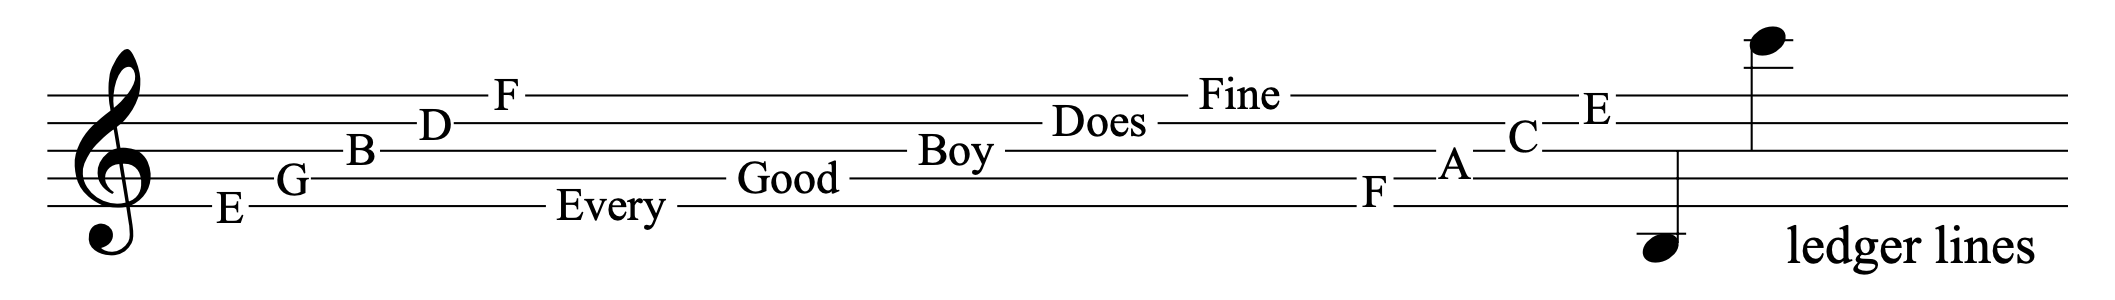
\includegraphics[width=\textwidth]{assets/staff}
    \caption{~The staff with a treble clef~\cite{music-theory}}\label{fig:staff}
\end{figure}


\section{Octave registers}\label{sec:octave-registers}

The note names used in music are \textit{ABCDEFG} (known as the ``musical alphabet'').
After G, note A returns, and \textit{ABCDEFG} occurs again.
An octave is a distance from any note to the same note in the next or previous register.
A piano also contains so-called \textit{accidentals} (special keys that raise or lower a note's pitch).
The piano keyboard with 88 notes consists of seven octaves (composed of seven notes and five accidentals) along with three extra notes and one extra accidental.~\cite{music-theory}

When learning about octave registers, we focus on note C for reasons that will soon become clear after learning about the major scale.
We use octave registers (C4, D5, \ldots) to specify the note's exact register.
The note C4 is known as \textbf{``middle C''} and is a vital reference point.
See the keyboard in the figure~\ref{fig:octave-registers}.~\cite{music-theory}

\begin{figure}
    \centering
    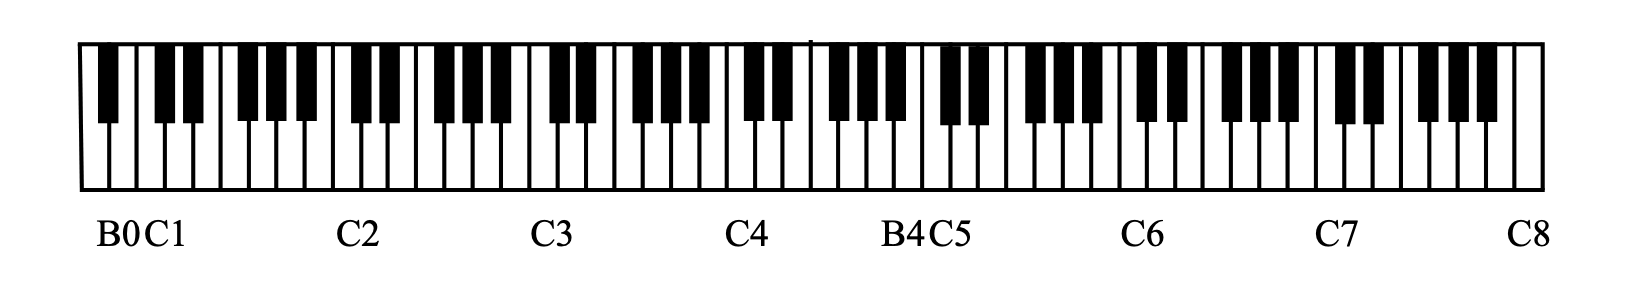
\includegraphics[width=\textwidth]{assets/octave-registers}
    \caption{~A piano with octave registers denoted~\cite{music-theory}}\label{fig:octave-registers}
\end{figure}

Notice that the register number changes after note B each time (e.g., B4 is followed by C5).
In the treble clef notation, middle C is placed on the \textit{ledger line} below the staff.
In the bass clef, the \textit{middle C} is placed on the \textit{ledger line} above the staff.
Both notations are visible in figure~\ref{fig:middle-c}.~\cite{music-theory}

\begin{figure}
    \centering
    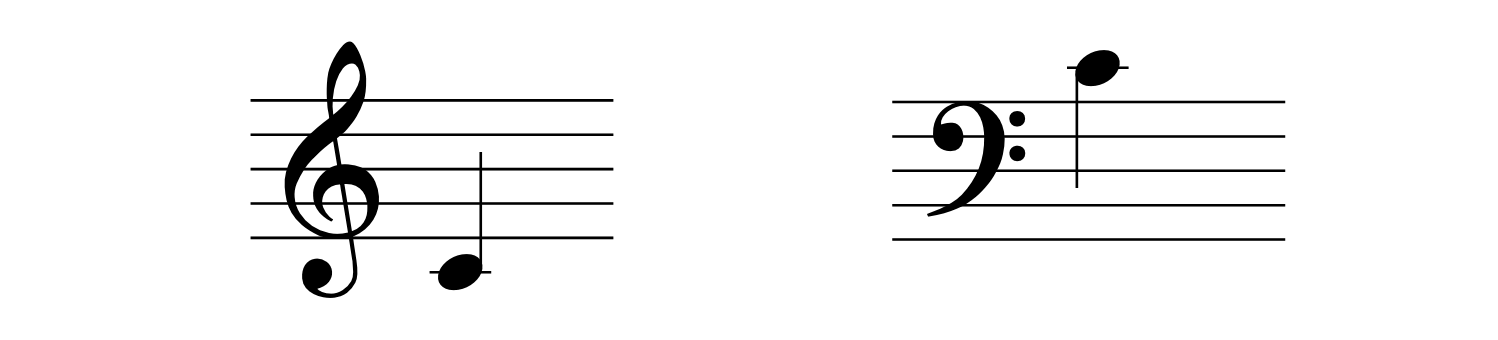
\includegraphics[width=\textwidth]{assets/middle-c}
    \caption{~Middle C (C4) in treble clef and bass clef~\cite{music-theory}}\label{fig:middle-c}
\end{figure}

When we join the treble and the bass clef together by a bracket, we create the so-called \textbf{grand staff}, how piano music is written.
An example of the \textbf{grand staff} is shown in figure~\ref{fig:grand-staff}.~\cite{music-theory}


\begin{figure}
    \centering
    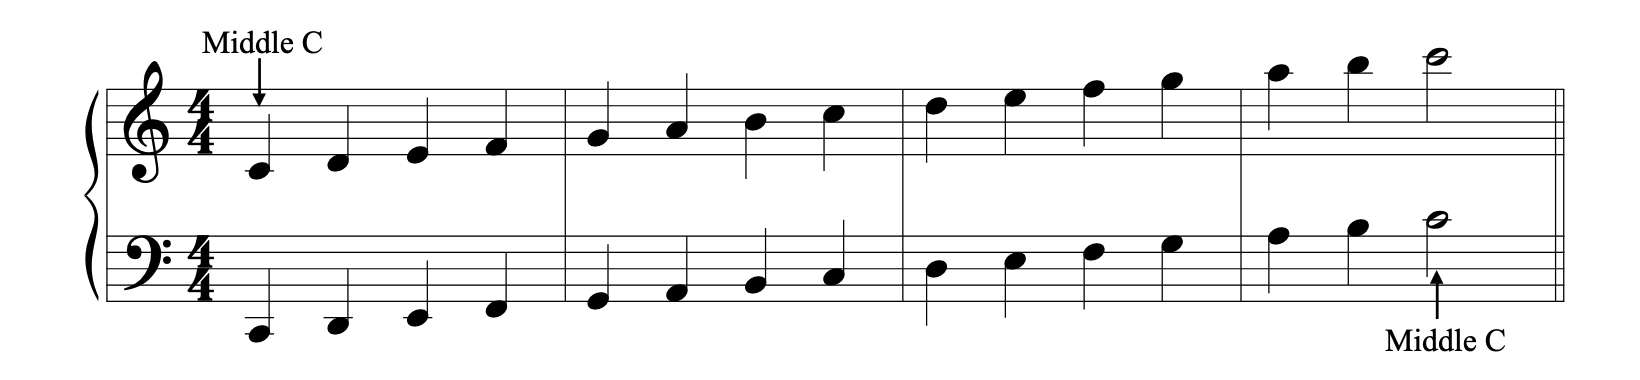
\includegraphics[width=\textwidth]{assets/grand-staff}
    \caption{~The grand staff~\cite{music-theory}}\label{fig:grand-staff}
\end{figure}


\section{Accidentals}\label{sec:accidentals}

Accidentals are characters that we use to modify the following note (either raise or lower the note pitch).
The following five symbols exist~\cite{music-theory}:

\begin{itemize}
    \item \textit{Sharp} symbol (\sh) raises pitch half a step
    \item \textit{Flat} symbol (\fl) lowers pitch half a step
    \item Double \textit{sharp} symbol (\musDoubleSharp) raises pitch two halves a step (a whole step)
    \item Double \textit{flat} symbol (\musDoubleFlat) lowers pitch two halves a step (a whole step)
    \item \textit{Natural} symbol (\na) cancels out accidentals previously applied in a measure of Major Key Signatures or Minor Key Signatures
\end{itemize}


\section{Half Steps and Whole Steps}\label{sec:half-whole-steps}

A half step on a piano keyboard is the distance from one note to the following immediate note.
A whole step composes of two half steps (figure~\ref{fig:half-whole-steps}).~\cite{music-theory}


\begin{figure}
    \centering
    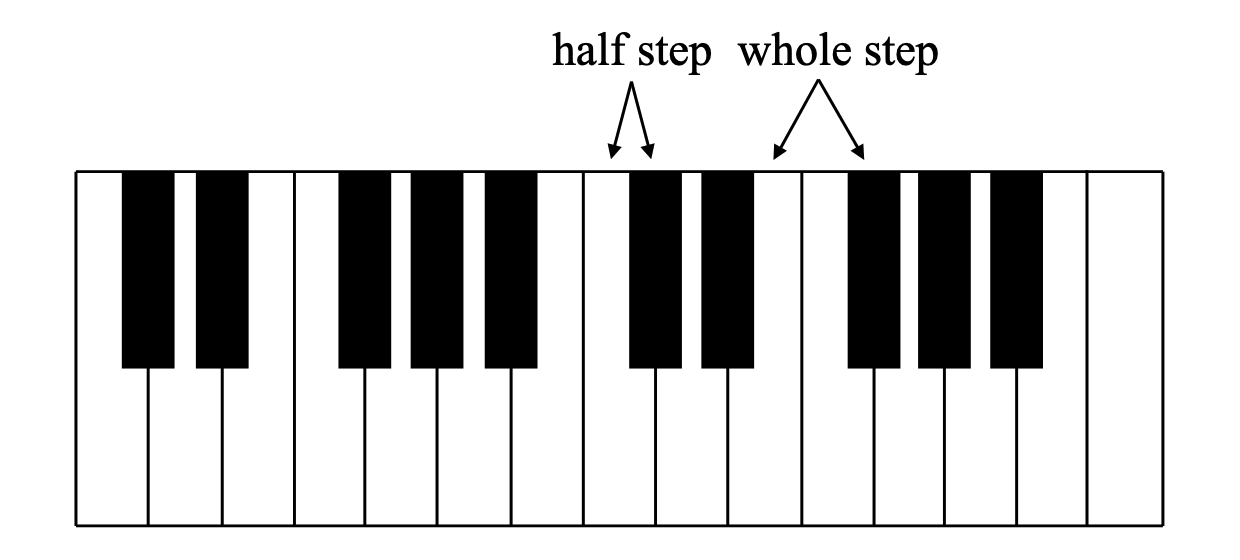
\includegraphics[width=0.78\textwidth]{assets/half-whole-steps}
    \caption{~The half step and whole step~\cite{music-theory}}\label{fig:half-whole-steps}
\end{figure}


\section{The Major scale}\label{sec:major-scale}

A specific sequence of whole and half steps is called a \textit{major scale}.
It is helpful to think of the pattern as consisting of two \textit{tetrachords}\footnote{\textit{``a tetrachord is a four-note scale segment''~\cite{music-theory}}} and a single whole step.
The lower \textit{tetrachord} is of the following pattern: whole step, whole step, half step.
A whole step then joins both \textit{tetrachords} together.
The upper \textit{tetrachord} consists of the same pattern as the lower one: whole step, whole step, half step.
If we use W for the whole step and H for the half step, we can write the major scale pattern as W--W--H, Whole–step connection, W--W--H.~\cite{music-theory}


\begin{figure}
    \centering
    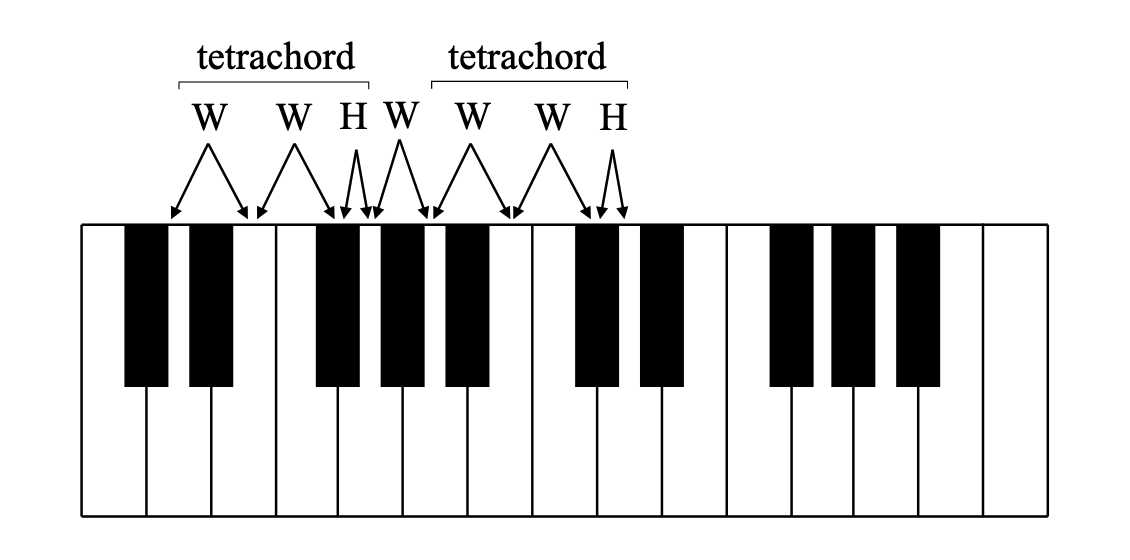
\includegraphics[width=0.8\textwidth]{assets/major-scale-keyboard}
    \caption{~The D major scale on a keyboard~\cite{music-theory}}\label{fig:major-scale-keyboard}
\end{figure}


\begin{figure}
    \centering
    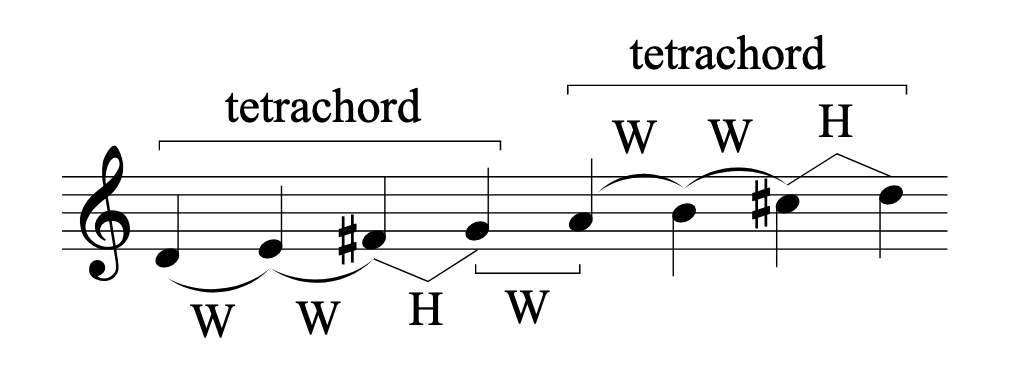
\includegraphics[width=0.84\textwidth]{assets/major-scale-staff}
    \caption{~The D major scale in treble clef~\cite{music-theory}}\label{fig:major-scale-staff}
\end{figure}

Note that all \textit{major scales} use the notes of the musical alphabet in order;
no notes get skipped, and no note occurs twice.
In figure~\ref{fig:major-scale-staff}, the first four notes are D--E--F\textsuperscript{\sh}--G, not D--E--G\textsuperscript{\fl}--G.
In D--E--G\textsuperscript{\fl}--G, G incorrectly occurs twice, and the F\textsuperscript{\sh} between E and G gets skipped.~\cite{music-theory}


\section{Major key signatures}\label{sec:major-key-signatures}

The key signature is a notation positioned next to the clef at the beginning of a piece or section.
We use it to hint which sharps or flats are in the piece's scale to prevent the composer from writing every sharp/flat from the scale each time it occurs.~\cite{music-theory}

There are \textbf{15} major \textit{key signatures}.
The key of \textit{C major has no sharps or flats} in the key signature, while the other key signatures can have between \textit{1 to 7 sharps} and \textit{1 to 7 flats}, resulting in the other 14 key signatures.
Notations of the major key signatures can be seen in figures 23 and 24 for sharps and flats, respectively.~\cite{music-theory}


\begin{figure}
    \centering
    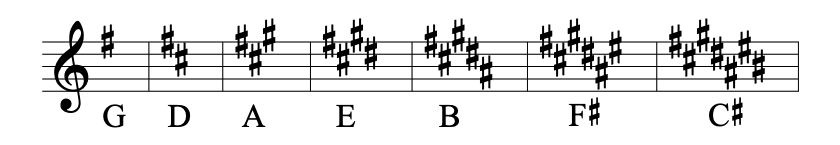
\includegraphics[width=\textwidth]{assets/major-signatures-sharps}
    \caption{~Major key signatures in sharps~\cite{music-theory}}\label{fig:major-signatures-sharps}
\end{figure}


\begin{figure}
    \centering
    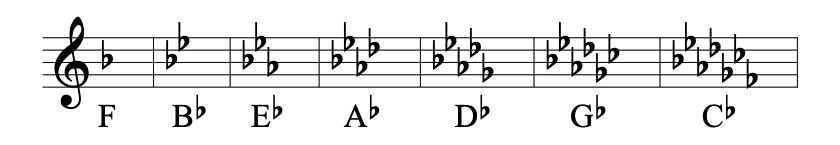
\includegraphics[width=\textwidth]{assets/major-signatures-flats}
    \caption{~Major key signatures in flats~\cite{music-theory}}\label{fig:major-signatures-flats}
\end{figure}

\textit{``A helpful learning device to remember the order of keys in relation to the order of sharps and flats is the \textbf{circle of fifths}.
As you ascend in fifths (clockwise), key signatures get one degree `sharper.'
    (C to G is a fifth because C=1, D=2, E=3, F=4, and G=5.)
    As you descend in fifths (counterclockwise), key signatures get one degree `flatter.'{''}}~\cite{music-theory}~(figure~\ref{fig:circle-of-fifths})


\begin{figure}
    \centering
    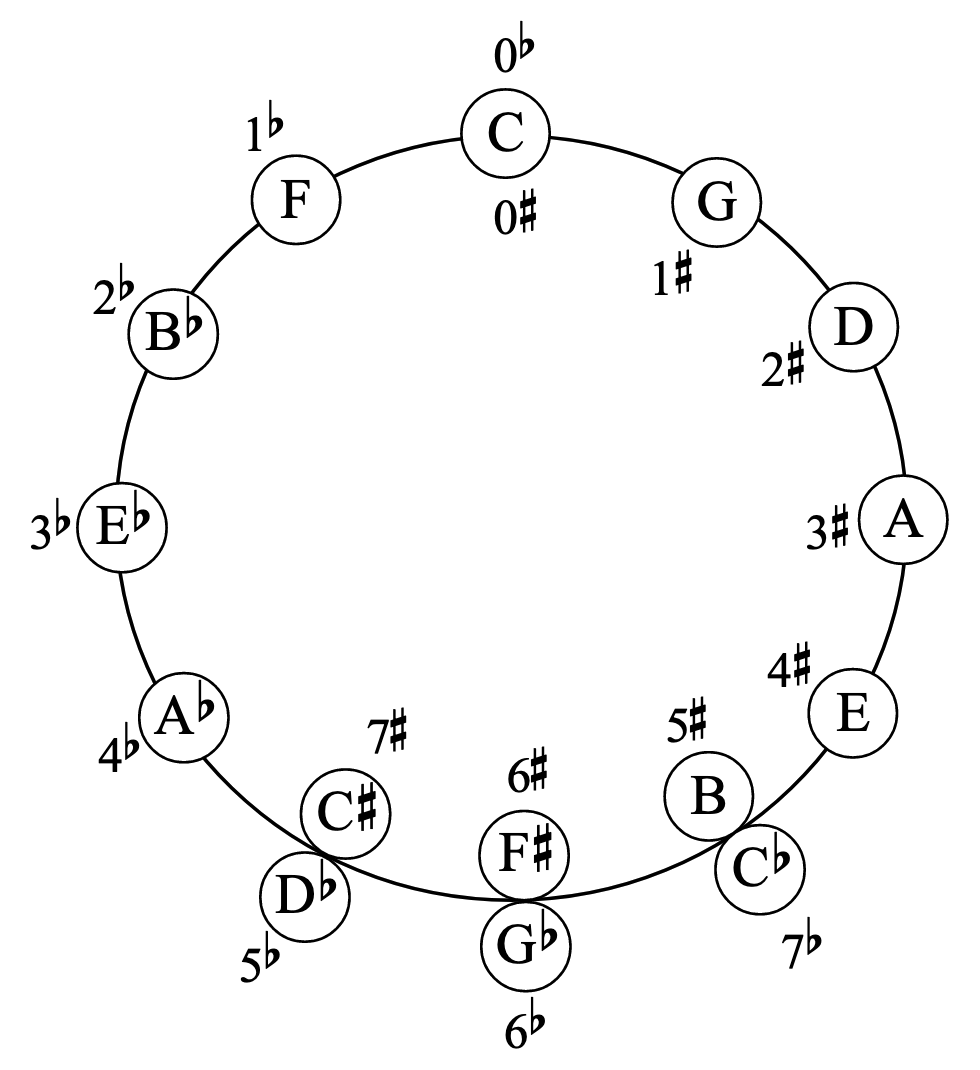
\includegraphics[width=0.6\textwidth]{assets/circle-of-fifths}
    \caption{~Circle of fifths in major keys~\cite{music-theory}}\label{fig:circle-of-fifths}
\end{figure}

Notice the overlapping keys at the bottom of the circle.
B major is enharmonically\footnote{pitches that are the same notes on a piano but are written differently on the staff} the same as C\textsuperscript{\fl} major, F\textsuperscript{\sh} major is enharmonically the same as G\textsuperscript{\fl} major, and C\textsuperscript{\sh} major is enharmonically the same as D\textsuperscript{\fl} major.~\cite{music-theory}


\section{Minor scales}\label{sec:minor-scales}

Alongside the \textit{major scale}, there are also three \textit{minor scales}: the \textit{natural minor scale}, the \textit{harmonic minor scale}, and the \textit{melodic minor scale}.
The \textit{melodic minor scale} has an ascending version, and a descending version that is the same as the \textit{natural minor scale}.
Both can be seen in figure~\ref{fig:minor-scale}.


\begin{figure}
    \centering
    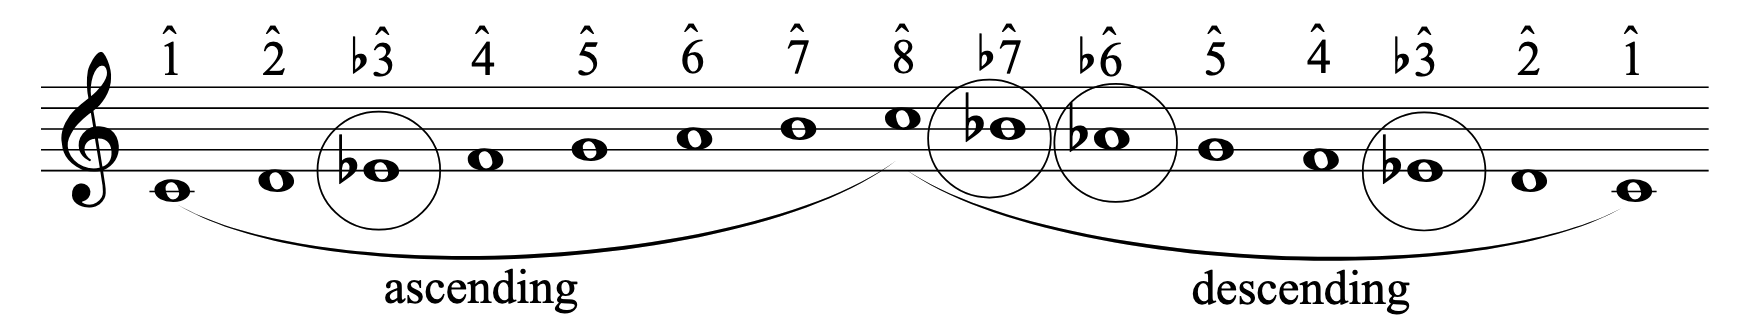
\includegraphics[width=\textwidth]{assets/minor-scale}
    \caption{~Melodic minor scale~\cite{music-theory}}\label{fig:minor-scale}
\end{figure}


\section{Minor key signatures}\label{sec:minor-key-signatures}

\textit{Minor key signatures} agree with the notes of the natural minor scale.
Since the C natural minor scale had E\textsuperscript{\fl}, A\textsuperscript{\fl} and B\textsuperscript{\fl} accidentals, the key signature of C minor has three flats, written in the order of flats (B\textsuperscript{\fl}, E\textsuperscript{\fl}, A\textsuperscript{\fl}).~\cite{music-theory}


\begin{figure}
    \centering
    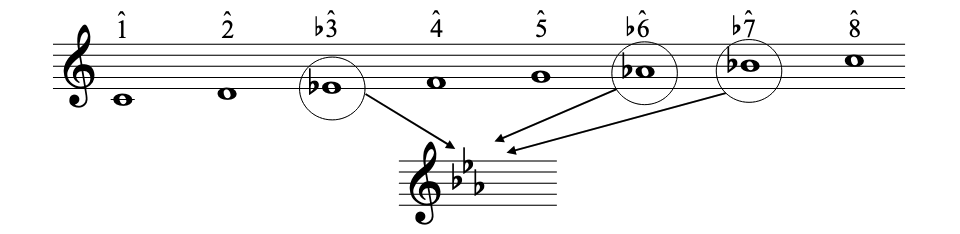
\includegraphics[width=\textwidth]{assets/natural-in-major}
    \caption{~Natural minor scale in major key signature~\cite{music-theory}}\label{fig:natural-in-major}
\end{figure}


\begin{figure}
    \centering
    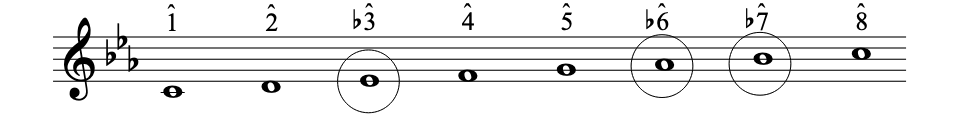
\includegraphics[width=\textwidth]{assets/natural-in-minor}
    \caption{~Natural minor scale in minor key signature~\cite{music-theory}}\label{fig:natural-in-minor}
\end{figure}


A \textit{minor key signature} will have three lowered notes—the third, sixth and seventh—related to the corresponding major key signature.
We use the term \textit{parallel minor} when referring to a minor scale (e.g., the parallel major of F minor is F major) with the same first scale degree (in this case C) as the major.
One method of figuring out a minor key signature is to add three flats (or subtract three sharps) to the parallel major key signature.
When writing below the five-line staff to designate keys, we use upper case for major keys and \textit{lowercase for minor keys}.
~\cite{music-theory}


\begin{figure}
    \centering
    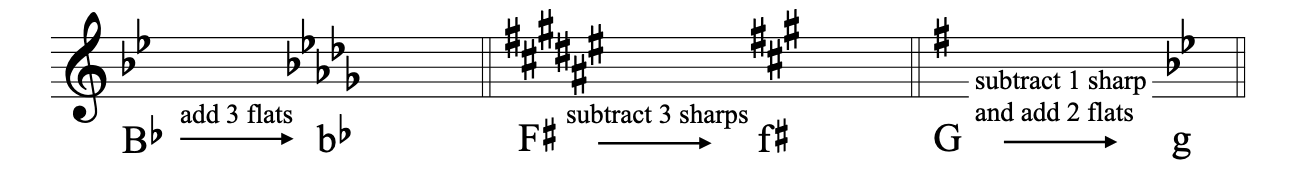
\includegraphics[width=\textwidth]{assets/parallel-minors}
    \caption{~Parallel minor keys signatures~\cite{music-theory}}\label{fig:parallel-minors}
\end{figure}

We also add figures of minor key signatures (figure~\ref{fig:minor-key-signatures}) and circle of fifths (figure~\ref{fig:circle-of-fifths-minor}) for minor scale for completeness.


\begin{figure}
    \centering
    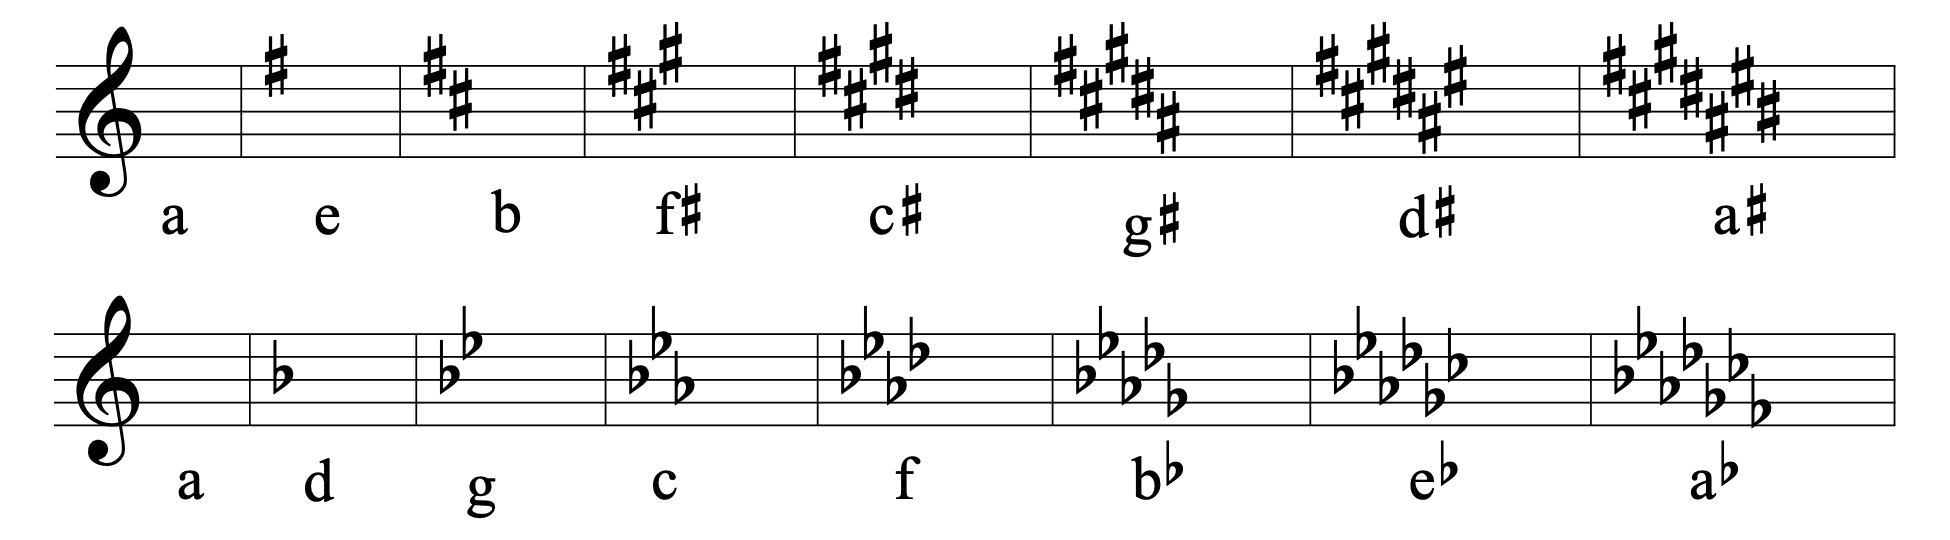
\includegraphics[width=\textwidth]{assets/minor-key-signatures}
    \caption{~Minor keys signatures~\cite{music-theory}}\label{fig:minor-key-signatures}
\end{figure}



\begin{figure}
    \centering
    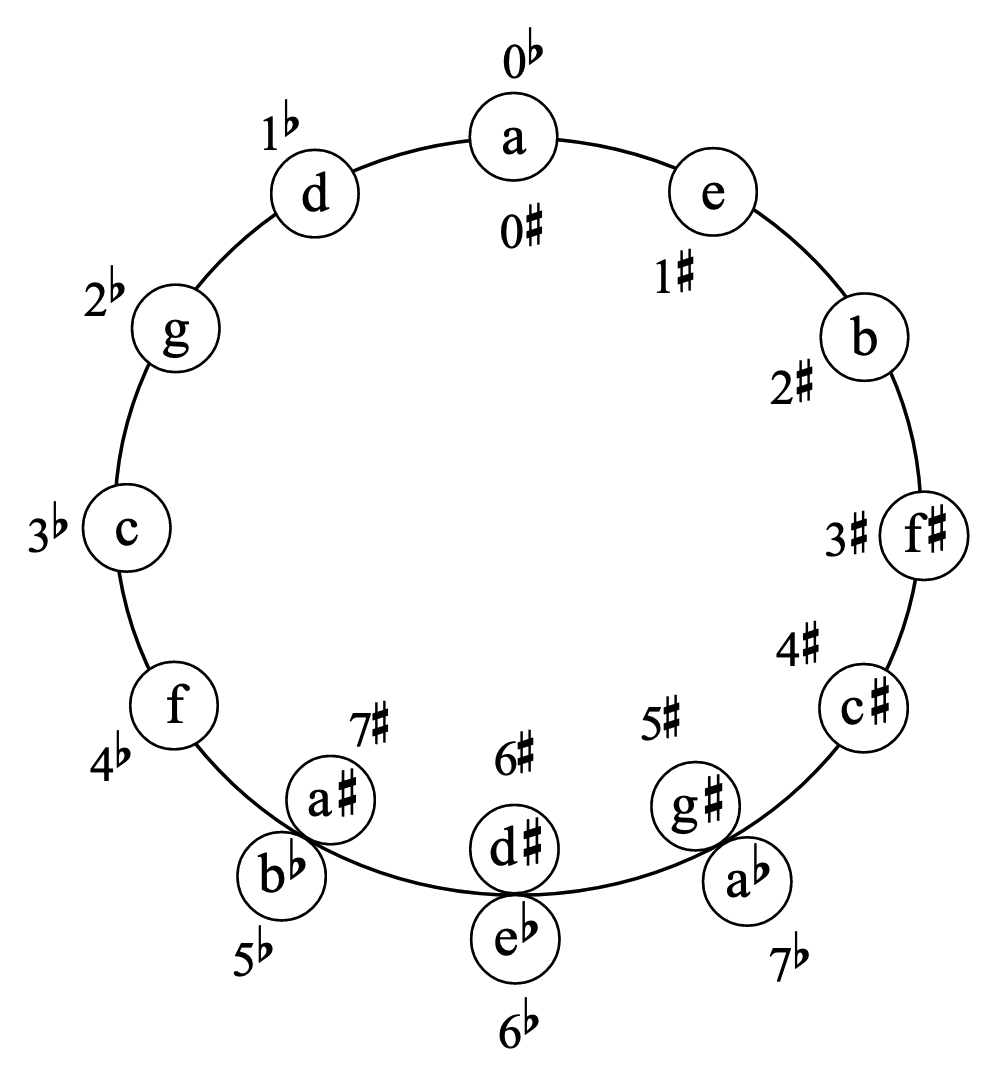
\includegraphics[width=0.6\textwidth]{assets/circle-of-fifths-minor}
    \caption{~Circle of fifths in minor keys~\cite{music-theory}}\label{fig:circle-of-fifths-minor}
\end{figure}


\section{Time signature}\label{sec:time-signature}


The staff can also contain a \textit{time signature} next to a clef.
We denote it as two stacked numbers;
the lower number is typically a number corresponding to a power of 2 and tells us the relative duration of a note, while the upper number hints at how many pulses (or \textit{beats}) we can expect per \textit{bar}\footnote{specified segment of time corresponding to the number of beats}.~\cite{music-theory}


\begin{figure}
    \centering
    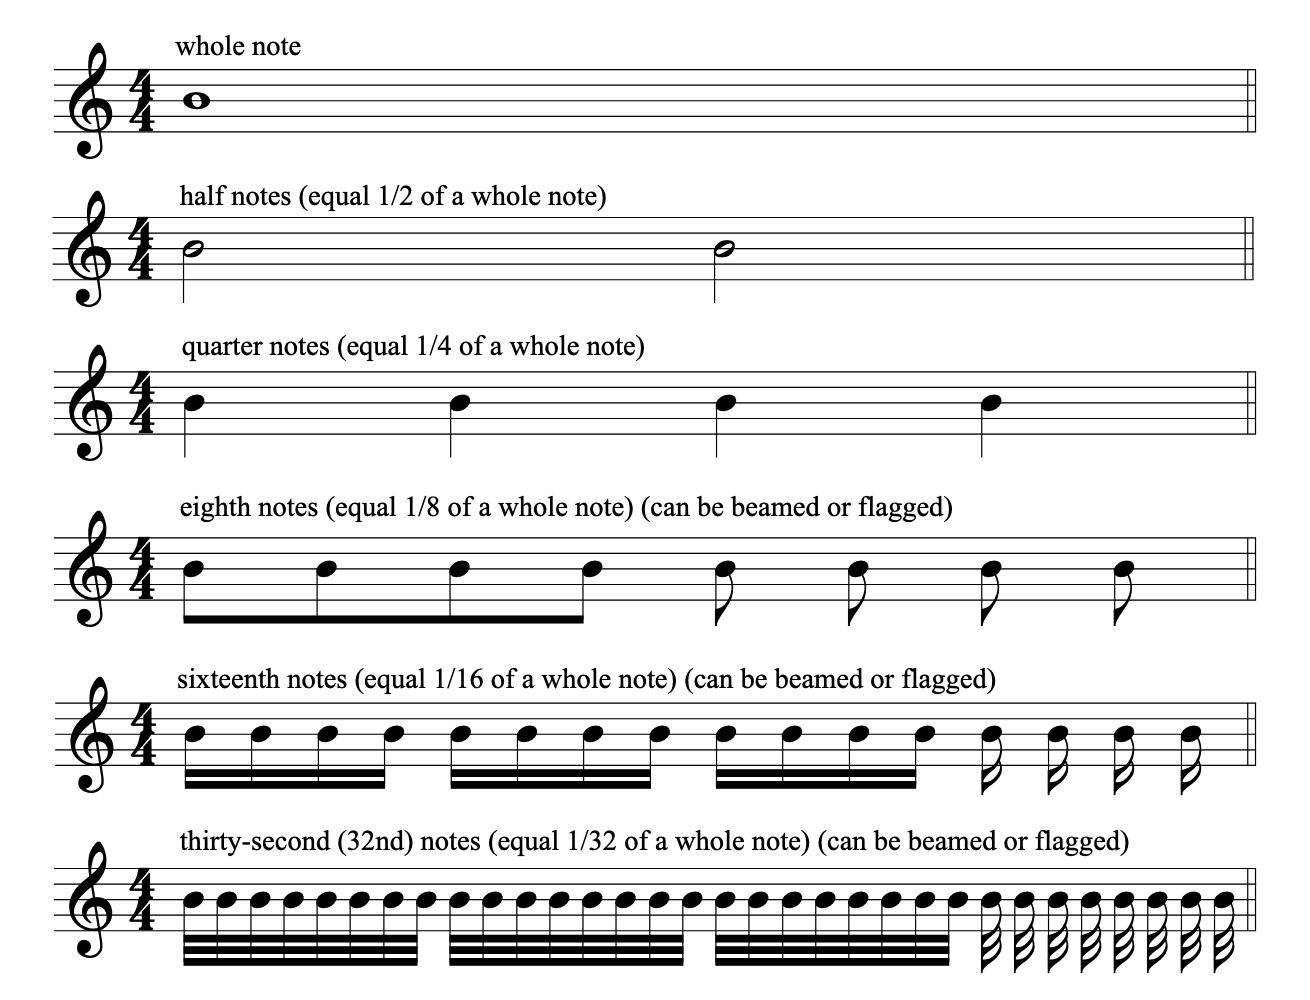
\includegraphics[width=0.8\textwidth]{assets/common-time-notes}
    \caption{~Different notes used for a common time~\cite{music-theory}}\label{fig:common-time-notes}
\end{figure}


\section{Durational symbols}\label{sec:durational-symbols}

The most common \textit{time signature} is $_{4}^{4}$ (also known as ``common time'').
It makes sense to introduce \textit{durational symbols} in the context of $_{4}^{4}$ time signature because a whole note takes up a full measure in $_{4}^{4}$, a half note takes up half a measure of $_{4}^{4}$, a quarter note takes up $\frac{1}{4}$ of a measure, and so on.


\begin{figure}
    \centering
    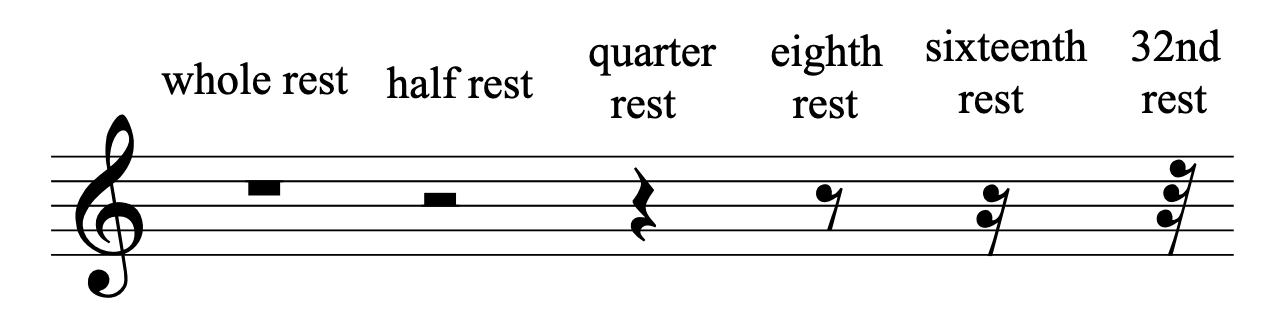
\includegraphics[width=0.9\textwidth]{assets/durational-symbols}
    \caption{~Durational symbols for rests~\cite{music-theory}}\label{fig:durational-symbols}
\end{figure}

Meter describes the number of beats in a measure (also called a bar) and how we typically divide the beats.
A beat is a basic pulse measured in music and thus the unit in which we think about music.
Pulse and beat are interchangeable.
The speed of a beat is called tempo.
We can state tempo in beats per minute (\textit{bpm}), such as 60bpm (where the rate of the beat would be equal to a second), or, in classical music, with terms like Allegro, Andante, and Adagio, sometimes in combinations with ``M.M.'' for Maelzel's Metronome.~\cite{music-theory}

Some meters have a special name;
meters with two beats in a bar are called \textit{duple}, three beats in a bar \textit{triple}, and four beats in a bar \textit{quadruple}.
Meter is described as \textit{simple} if the beats are normally divided into two parts and \textit{compound} if the beats are normally divided into three parts.~\cite{music-theory}



% Automated music generation
%---------------------------------------------------------------


\addcontentsline{toc}{chapter}{Automated music generation}
\markboth{Automated music generation}{Automated music generation}

\begin{chapterabstract}
    When talking about \textit{automated music generation}, we may want to distinguish between \textit{composition assistance} (software that is not generating the music from scratch but instead helps the composer incrementally with suggestions, auto-completion, etc.) and \textit{autonomous music generation} (which takes over the whole music composing process and users are restricted just to parametrization of the generation process).
    In this chapter, we will focus on the latter.
    We will briefly go over the history of the music generation and then move on to modern techniques utilizing machine learning techniques.~\cite{music-generation-history}
\end{chapterabstract}


\section{Pre-computer techniques}\label{sec:pre-computer-techniques}

First experimentations with \textit{algorithmic composition} took place in the late 15th century by employing \textbf{"canonic composition."}~\cite{brief-history-of-algo-composition}

\textit{``The prevailing method was to write out a single voice part and to give instructions to the singers to derive the additional voices from it.
The instruction or rule by which these further parts were derived was called a canon, which means `rule' or `law.' For example, the second voice might be instructed to sing the same melody starting a certain number of beats or measures after the original;
the second voice might be an inversion of the first or it might be a retrograde [etc.]''}~\cite{history-of-western-music}

These \textit{rules} of imitation and manipulation form an \textit{algorithm} by which performers unfold the music.
In this automatical process, we see a clear removal of the composer from a large portion of the compositional process: the composer himself only invents a core of the music, a single melody or section.~\cite{brief-history-of-algo-composition}

\textit{Wolfgang Amadeus Mozart} experimented with automated composition techniques using the so-called \textit{Musikalisches Wurfelspiel} (``musical dice game'').
The game worked by joining several predefined musical segments selected by dice roll.
This simple form of \textit{stochastic} algorithmic composition left the creative decisions in the hands of chance, letting the dice roll decide what notes to use.~\cite{brief-history-of-algo-composition}


\section{Use of computers}\label{sec:use-of-computer}

There are three possible approaches when using a computer to generate a composition:
\begin{itemize}
    \item Stochastic
    \item Rule-based
    \item Artificial intelligence
    % TODO: describe the items
\end{itemize}

The \textit{stochastic} way involves \textit{randomness} and can be as simple as Mozart's \textit{Musical dice game} we already briefly touched upon;
however, we can also use more complex methods like \textit{statistical theory} and \textit{Markov chains}.
Many creative decisions are merely left to chance when generating a composition using the stochastic method.
Another example of non-computer-oriented stochastic composition can be found in Karlheinz \textit{Stockhausen's Klaveirstucke XI}, in which the sequence of various fragments of music is to be performed by a pianist in random order.~\cite{brief-history-of-algo-composition}

\subsection{Markov chains}\label{subsec:markov-chains}

So-called \textit{Markov chains} are a major technique for generating musical compositions using stochastics.
We define the Markov chain using a simple sequence of random variables $X_1, X_2, X_3, \ldots, X_i$\footnote{the index $i$ in this context is sometimes referred to as the time}; we call this sequence a \textit{stochastic process}.
For this process to be the Markov chain, the following equivalence must be true:
\[ [X_i\rvert X_1, \ldots, X_{i-1}] \sim [X_i\rvert X_{i-1}] \]
In this context, the equivalence means that the \textit{probability distribution} on the left-hand side is equivalent to the probability distribution on the right-hand side.
For a fixed value of $i$, $X_i$ is called the state of the Markov chain.
The equivalence implies that the value of $i\textsuperscript{th}$ state is purely dependent on the immediately previous state, a trait also called \textit{memoryless}.~\cite{markov-chains}

Markov chains are primarily represented in two ways a \textit{transition matrix} (figure~\ref{fig:markov-chain-matrix}) or a \textit{directed graph} (figure~\ref{fig:markov-chain-graph}).
The transition matrix $M$ is a matrix with dimensions $n$ by $n$, where $n$ is the number of different states the Markov chain maintains.
The $M_{a,b}$ value then represents $\mathcal{P}(b \rvert a)$, the probability of transition from the state $a$ to state $b$.
This representation is practical for use in computers.
The directed graph is a good representation for visualization;
each \textit{vertex} represents a state, and the \textit{directed edges} represent the probability of a transition between two states.~\cite{markov-chains}

\begin{figure}
    \centering
    \[
        \begin{blockarray}{cccc}
            & \text{Sunny}     & \text{Windy}     & \text{Rainy} \\
            \begin{block}{c(ccc)}
                \text{Sunny}     & 0.6     & 0.3     & 0.1 \\
                \text{Windy}     & 0.7     & 0       & 0.3 \\
                \text{Rainy}     & 0.5     & 0.2     & 0.3 \\
            \end{block}%
        \end{blockarray}%
    \]
    \caption{~Markov chain represented by transition matrix~\cite{markov-chains}}\label{fig:markov-chain-matrix}
\end{figure}

\begin{figure}
    \centering
    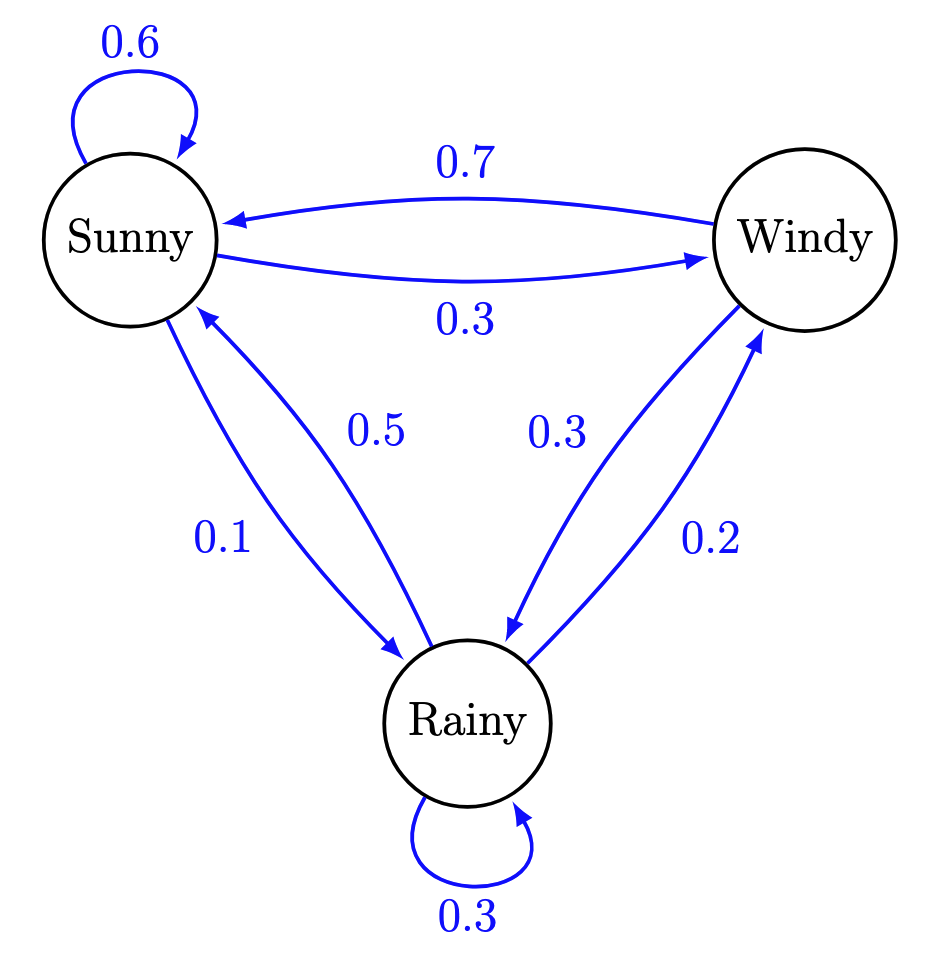
\includegraphics[width=0.5\textwidth]{assets/markov-chain-graph}
    \caption{~Markov chain represented by directed graph~\cite{markov-chains}}\label{fig:markov-chain-graph}
\end{figure}

\subsubsection{Generating music}\label{subsubsec:generating-music}

Once we have the Markov chain defined, we can use it to generate music in a simple manner;
we want to create a model that will contain sound objects (notes or chords and their duration) as states and probabilities of transitions between them.
We do this by using existing music pieces and using them as training input.
We compose the states by extracting all different sound objects occurring in the training pieces.
We can compute the transition probabilities by gathering all possible \textit{bigrams} (sequences of two adjacent objects).
The probability of transition from the state $a$ to state $b$ is then computed by following division $\mathcal{P}(b \rvert a) = \frac{\# ab}{\# ac}$, where $ab$ represents bigrams of sound object $a$ followed by sound object $b$, and $ax$ represents \textit{all bigrams} starting with the object $a$.
Using this method we compose the whole transition matrix.

With the transition matrix available, we can move on to the music generation itself.
In order to utilize the matrix for generating transitions, we first need to select the first sound object the musical piece will start with.
We can do that by manually picking the desired sound object, or we can generate it randomly by composing a vector of probabilities of starting sound objects, where the probability of each object being the starting object is the number of times it was starting object in training musical pieces divided by the total number of training musical pieces.
So to generate the piece, we select starting object from the initial vector (the likelihood of selecting an object is determined by its computed probability).
Then for every other state, we receive the vector of probabilities by using a row of the transition matrix corresponding to the current state.
We iteratively continue until we are satisfied with the length of a piece.~\cite{markov-chains}

\subsection{Rule-based music generation}\label{subsec:rule-based}

Music theory traditionally describes rules that help to direct the compositional process.
While composers regularly break those rules, they can be successfully used to implement a system for generating music.
One of the examples would be the \textit{Illiac Suite}, composed in 1957 by professors \textit{Lejaren Hiller} and \textit{Leonard Issacson}, where the rule-based system was used to help generate the first two movements.~\cite{computational-creativity}

\textit{``The general idea is to use screening rules to accept or reject randomly generated pitches and rhythms.
Probability distribution and Markov processes can also be found in the suite.''}~\cite{illiac-suite}

\subsubsection{Formal Grammars}\label{subsubsec:formal-grammars}

In the 1950s, \textit{Noam Chomsky} introduced the concept of \textit{Generative Grammars}, a tool for analyzing language that became highly influential in linguistic studies.
In a Generative Grammar, two alphabets of \textit{terminal} and \textit{non-terminal symbols} are used, along with a set of \textit{rewriting rules} given over the union of these two alphabets that allow transforming non-terminal symbols (or string of non-terminal and terminal symbols) into other symbols (both terminals and non-terminals).
The generated \textit{language} is the set of all possible strings of terminal symbols generated from a special starting variable (usually called $S$) and applying any number of rewriting rules in sequence.
These Grammars can be seen as an implementation of the beforementioned rule-based systems.~\cite{computational-creativity}

\textit{Lindenmayer Systems} (L-Systems) are a variant of Generative Grammars used for music generation;
the difference from Chomsky's Grammars is that they implement \textit{parallel rewriting}, applying all the rewriting rules at once instead of only one at a time.
This characteristic makes these systems less inclined to generate sequential data, like simple melodies, and have been used to generate stunning visual effects.
When applied to music generation, a common approach was to map visual data generated by \textit{L-systems} to score information or to a sequence of musical segments.~\cite{computational-creativity}

One of the most influential researchers of rule-based music generation is \textit{Ebcioǧlu}, who implemented a custom logic language that he used to create \textsl{CHORAL}, a system for the generation of Bach-like chorales that uses some 350 rules for harmonization and generation of melodies~\cite{ebcioglu}.
The hardship of designing such a system lies in the complexity of explicitly coding enough rules, many of which often do not have a formal definition in musicology literature.~\cite{computational-creativity}


\subsection{Artificial intelligence}\label{subsec:artificial-intelligence-music-generation}

\textit{``Artificial Intelligence (AI) is the property of machines, computer programs and systems to perform the intellectual and creative functions of a person, independently find ways to solve problems, be able to draw conclusions and make decisions.''}~\cite{about-ai}

AI is a buzzword that contains two main branches, the original \textit{symbolic AI} and \textit{machine learning}.
The symbolic AI are systems where we capture knowledge using formal mathematical logic, genetic algorithms, state-space search, automated planning,~\ldots~.
The machine learning AI builds models with a set of hidden internal parameters we are trying to fine-tune so that the model performs well on predefined metrics;
this optimization process is called learning.
In this thesis, we will specifically focus on \textit{artificial neural networks}, which are subset of ML techniques.

The increased computational power of computers and the widespread general-purpose GPU programming recently made \textit{deep learning}\footnote{use of ANNs with more than three hidden layers} techniques extremely popular, with applications spanning from \textit{NLP} to \textit{image processing} to \textit{music generation}.

While the interest in these algorithms grew exponentially in the last decade, the first music generation system to use ANNs was that of Peter M. Todd\cite{first-ann-mgs}, who used a three-layered \textit{Recurrent Neural Network} (RNN) to generate monophonic melodies.
Recurrent Networks reuse the results of the computations from previous steps every time a new input is fed, allowing them to encode temporal sequences.
Still, standard feed-forward networks are also an option for music generation.
There is also room for standard feed-forward networks: in 1991, J. P. Lewis trained a network\cite{feed-forward-ann-mgs} with musical patterns ranging from random to well-constructed to learn a measure of ``musicality'' used by his music generation system to select pleasing compositions.

As mentioned, RNNs are a popular choice for music generation.
In particular, \textit{LSTMs}\cite{LSTMs} are a special variant of recurrent networks that use gates to decide the amount of information taken from novel input and what is maintained from older inputs, hence the memory.
The first LSTM used for music generation was applied to blues improvisation\cite{LSTM-mgs}.
Another deep learning approach is that of Generative Adversarial Networks (GANs)\cite{gans};
the concept behind this method is to train two networks at the same time, one generates musical compositions imitating what is learned from real-world examples, and the other tries to discriminate between original and imitated compositions.
As one network gets better, the other must improve as well in order to ``beat'' the other network (therefore making them ``Adversarial'').


 % include `text.tex' from `text/' subdirectory

    \appendix\appendixinit % do not remove these two commands

    \chapter{Appendix}

\begin{figure}
    \centering
    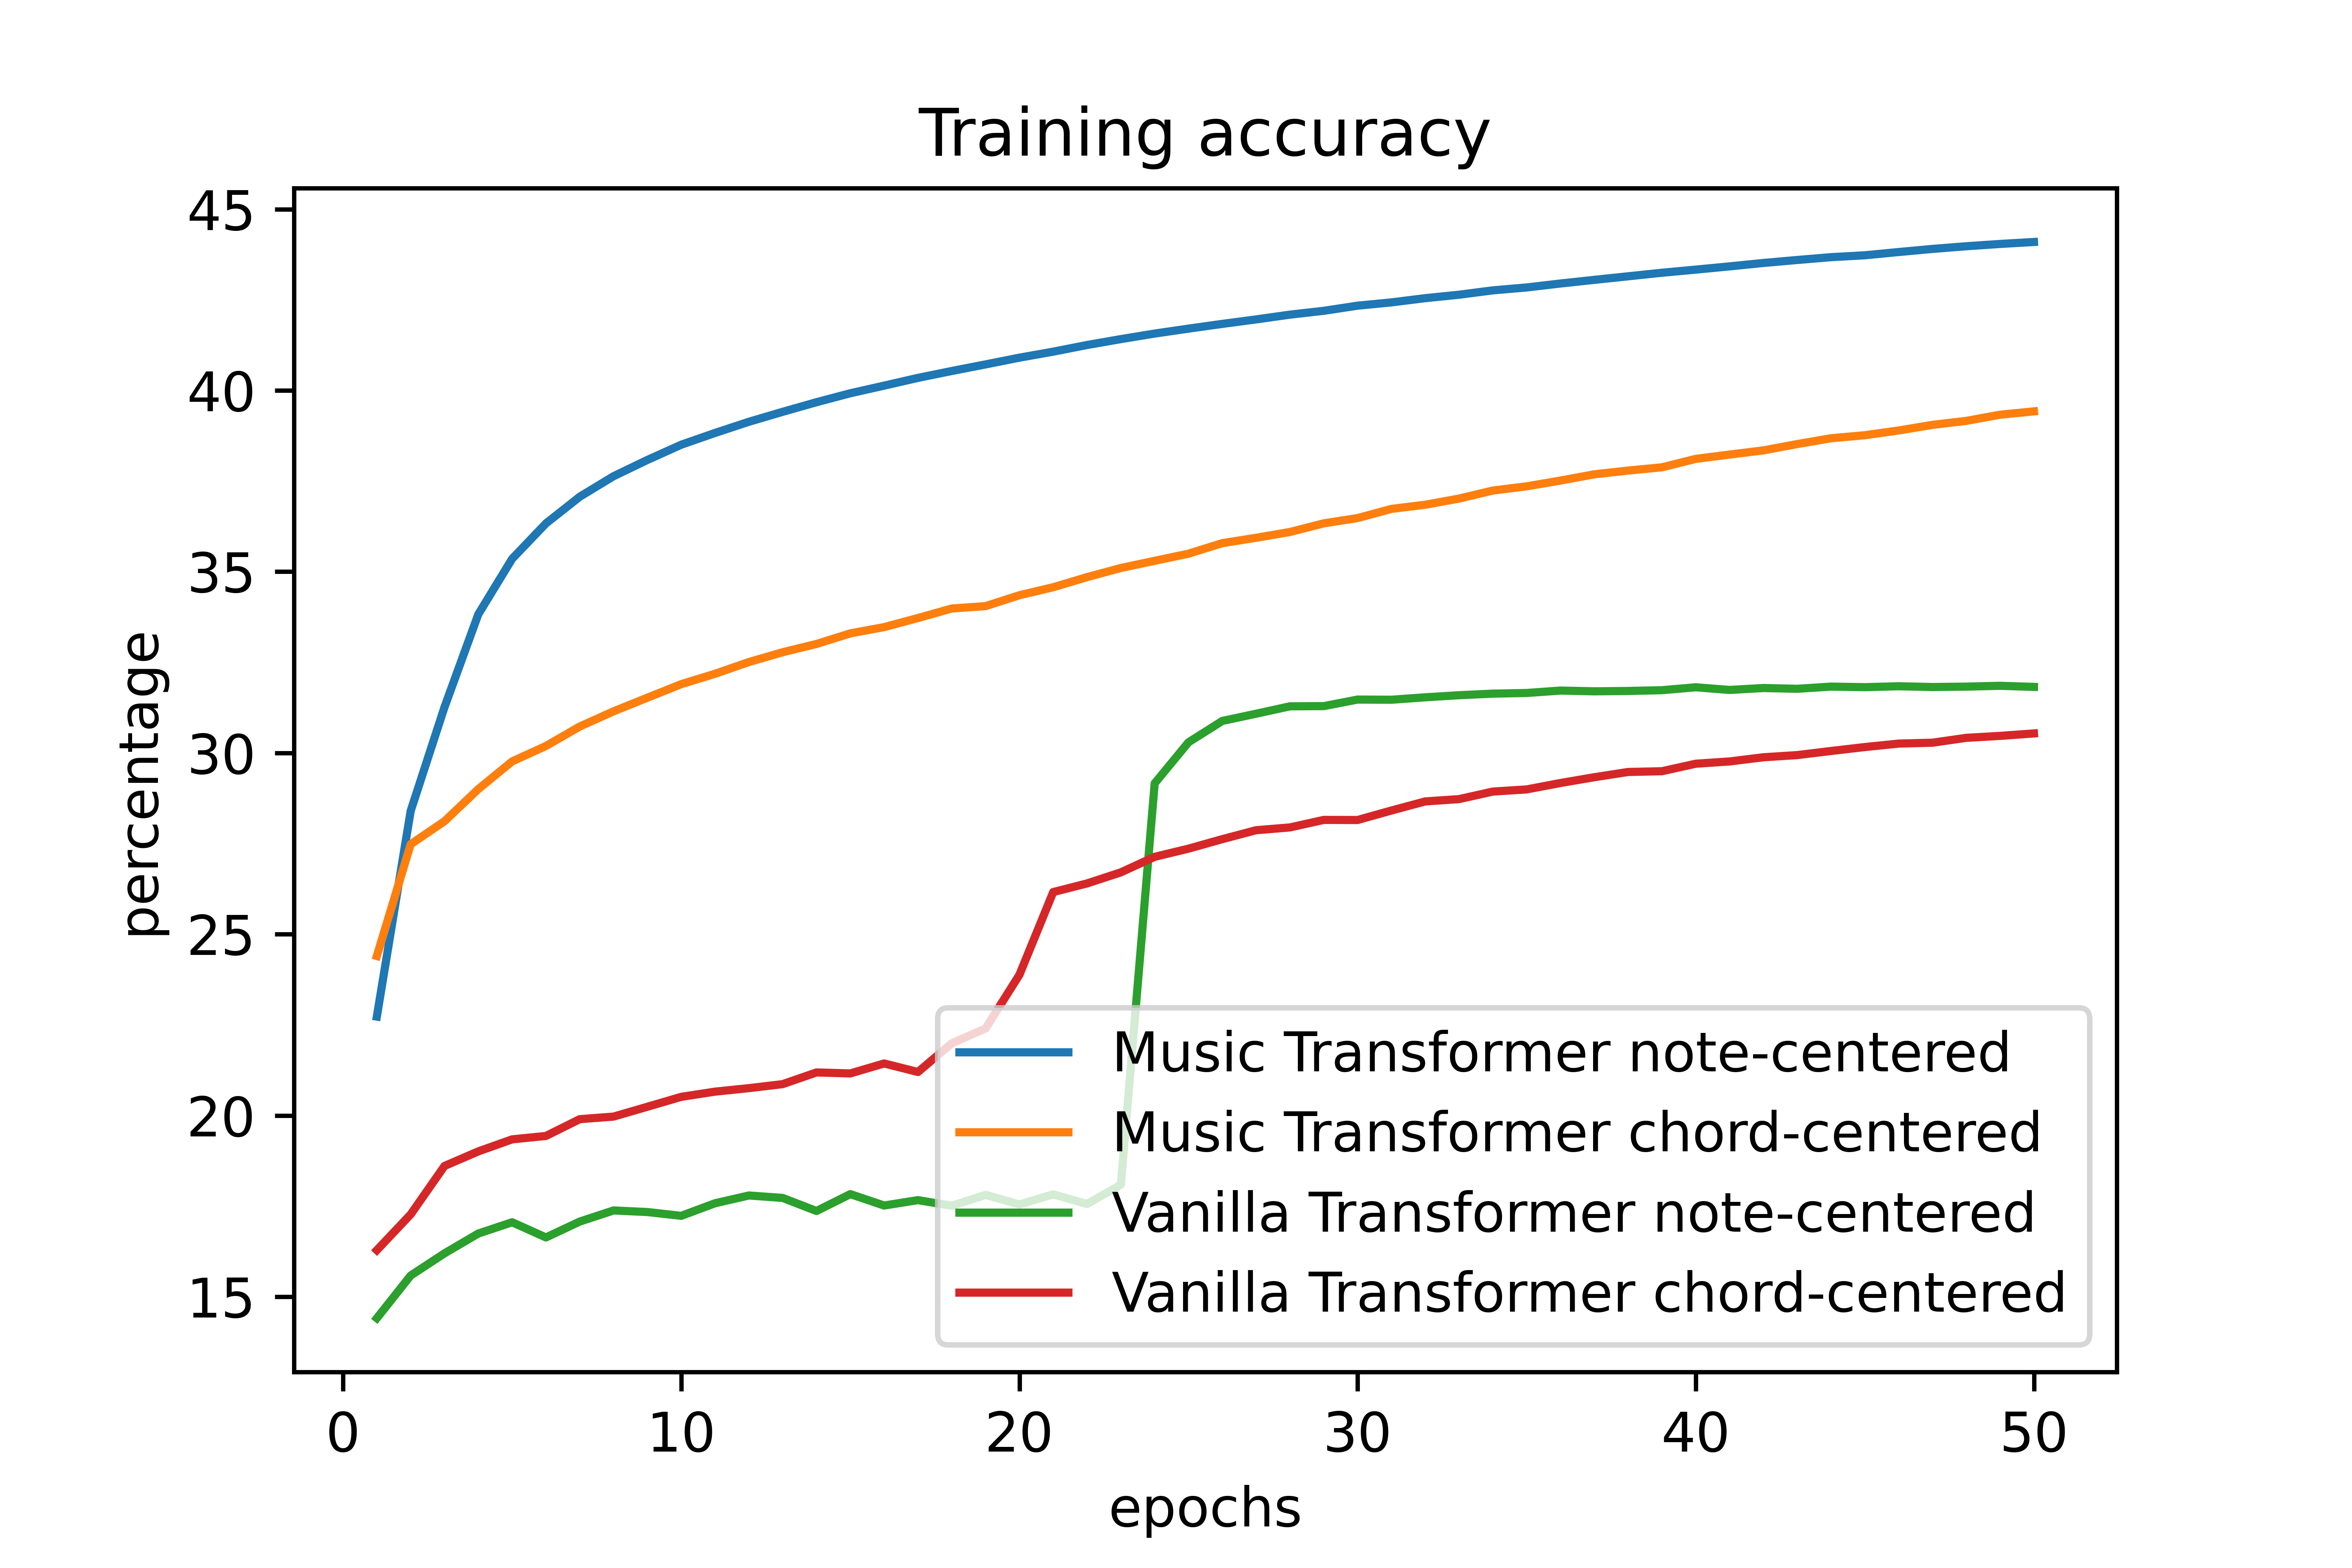
\includegraphics[width=0.8\textwidth]{assets/training-accuracy}
    \caption{~Accuracy of models on training set}\label{fig:appendix-training-accuracy}
\end{figure}
\begin{figure}
    \centering
    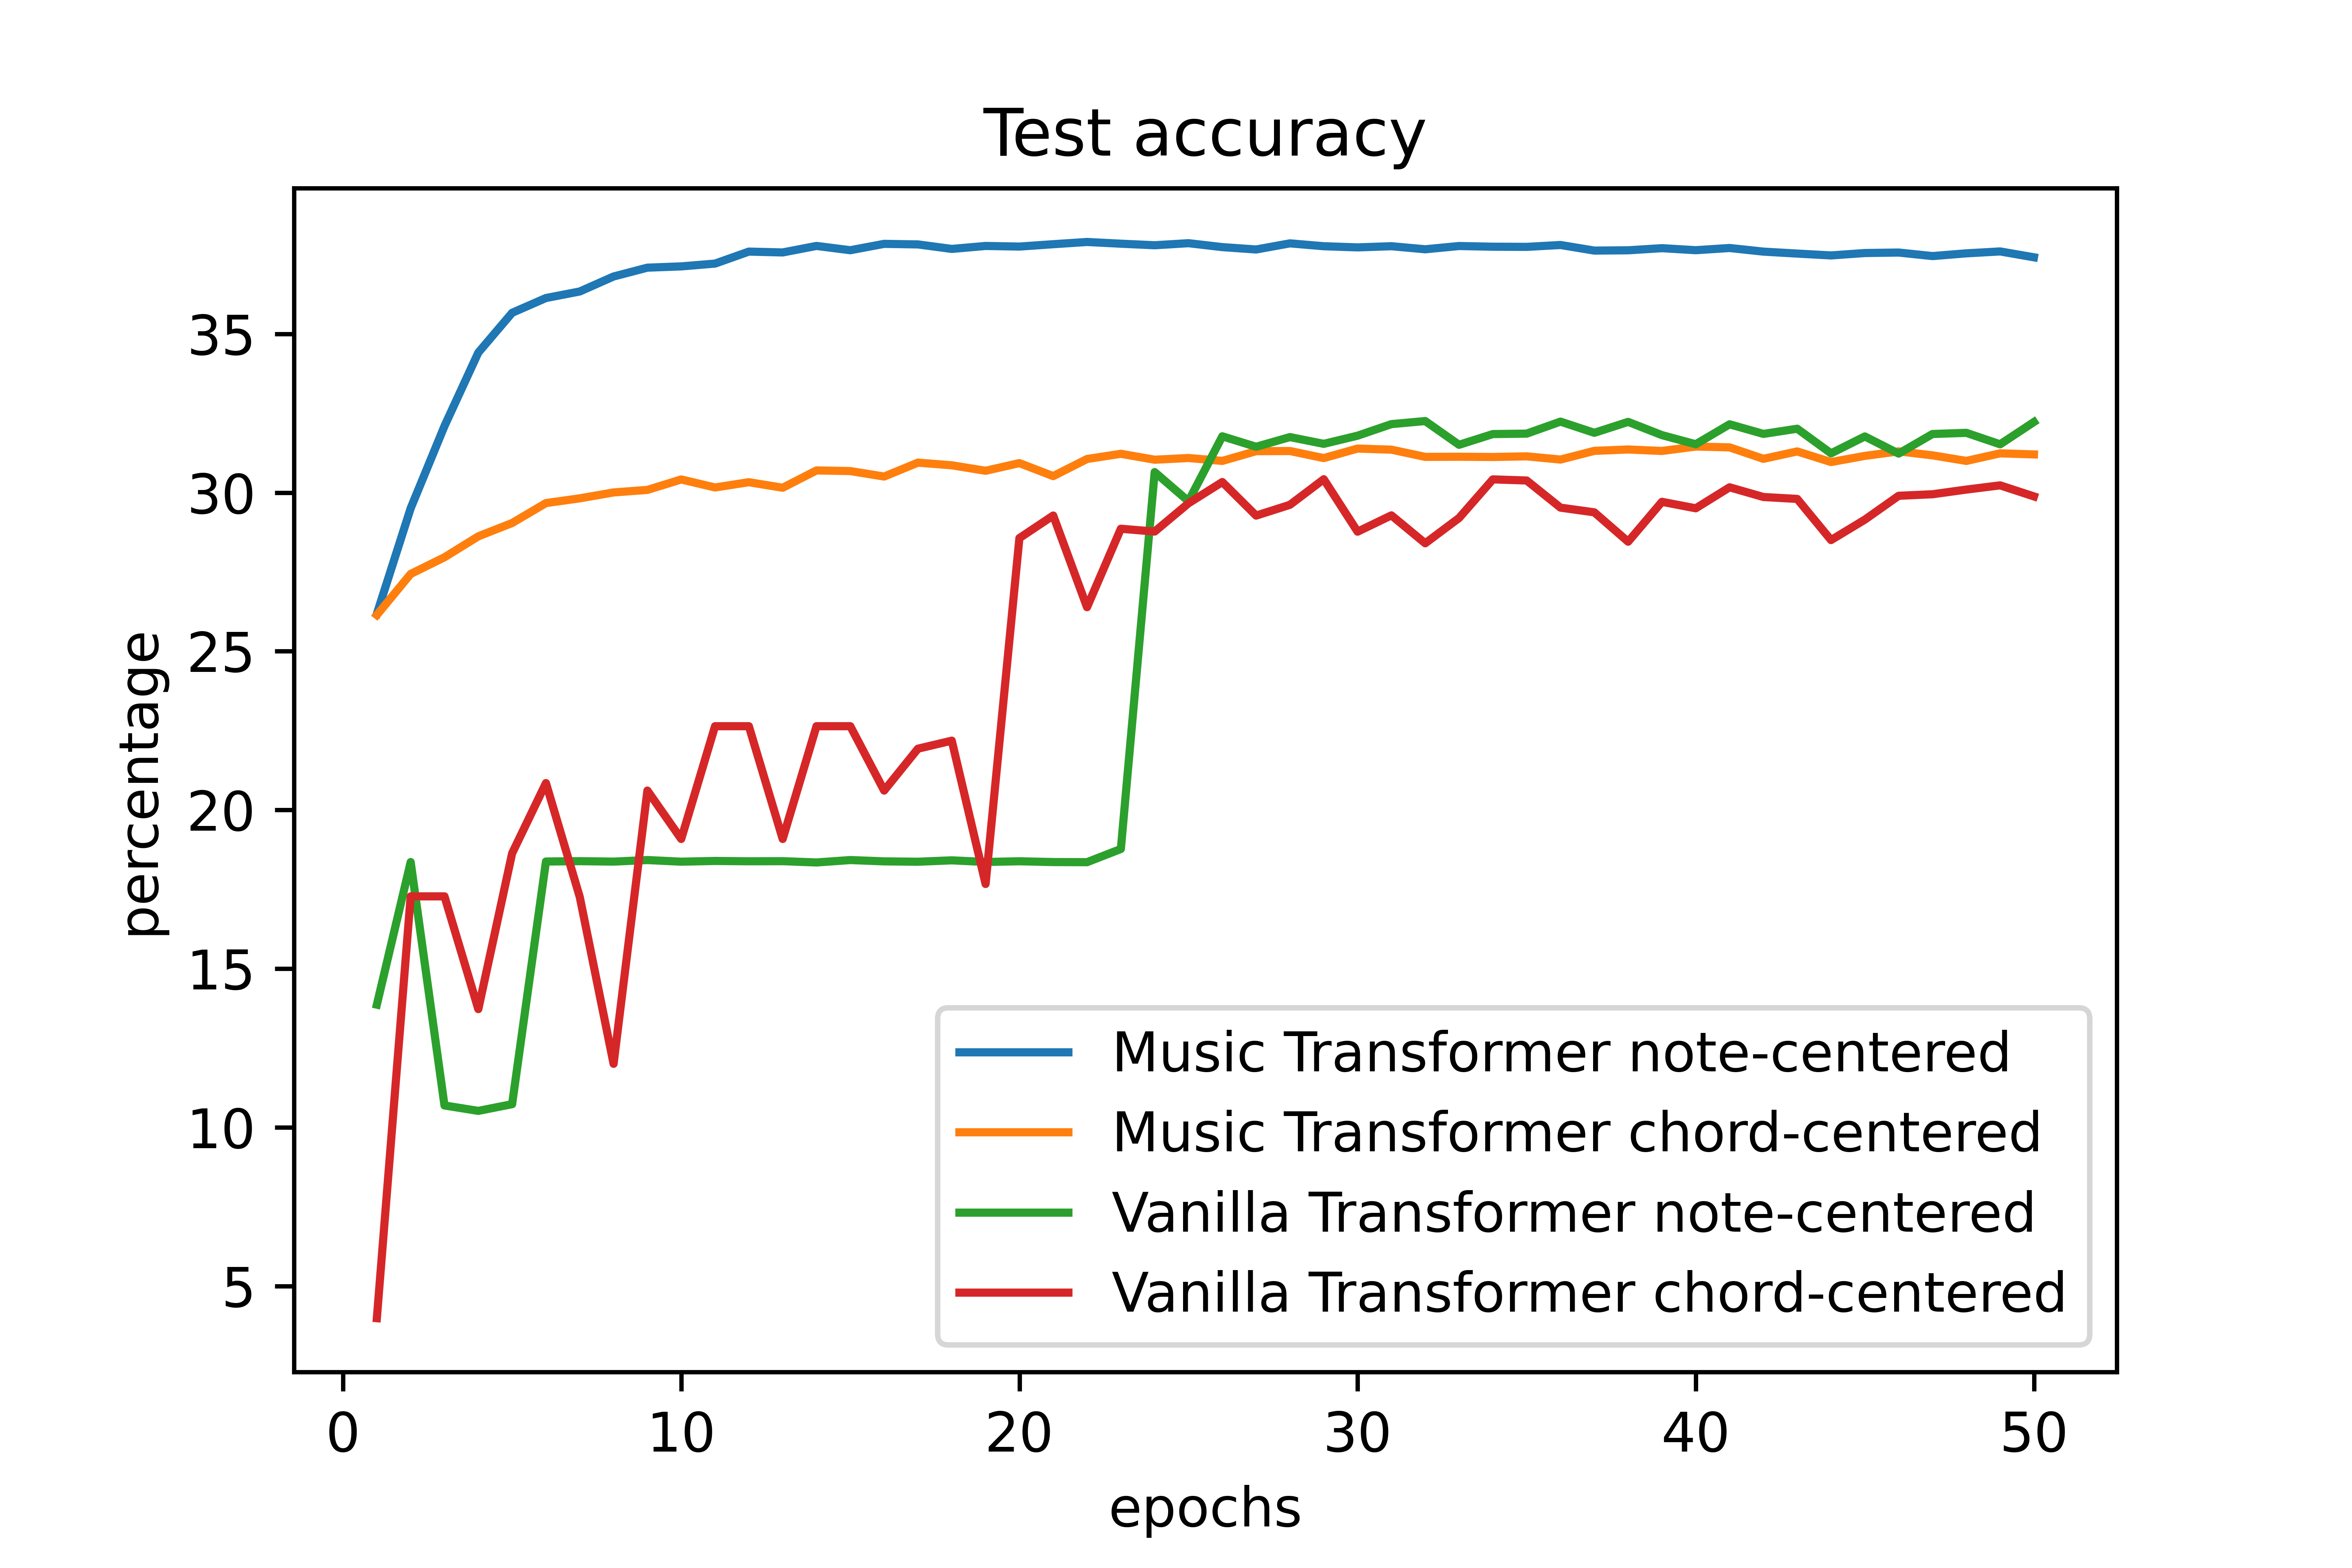
\includegraphics[width=0.8\textwidth]{assets/test-accuracy}
    \caption{~Accuracy of models on test set}\label{fig:appendix-test-accuracy}
\end{figure}

\begin{figure}
    \centering
    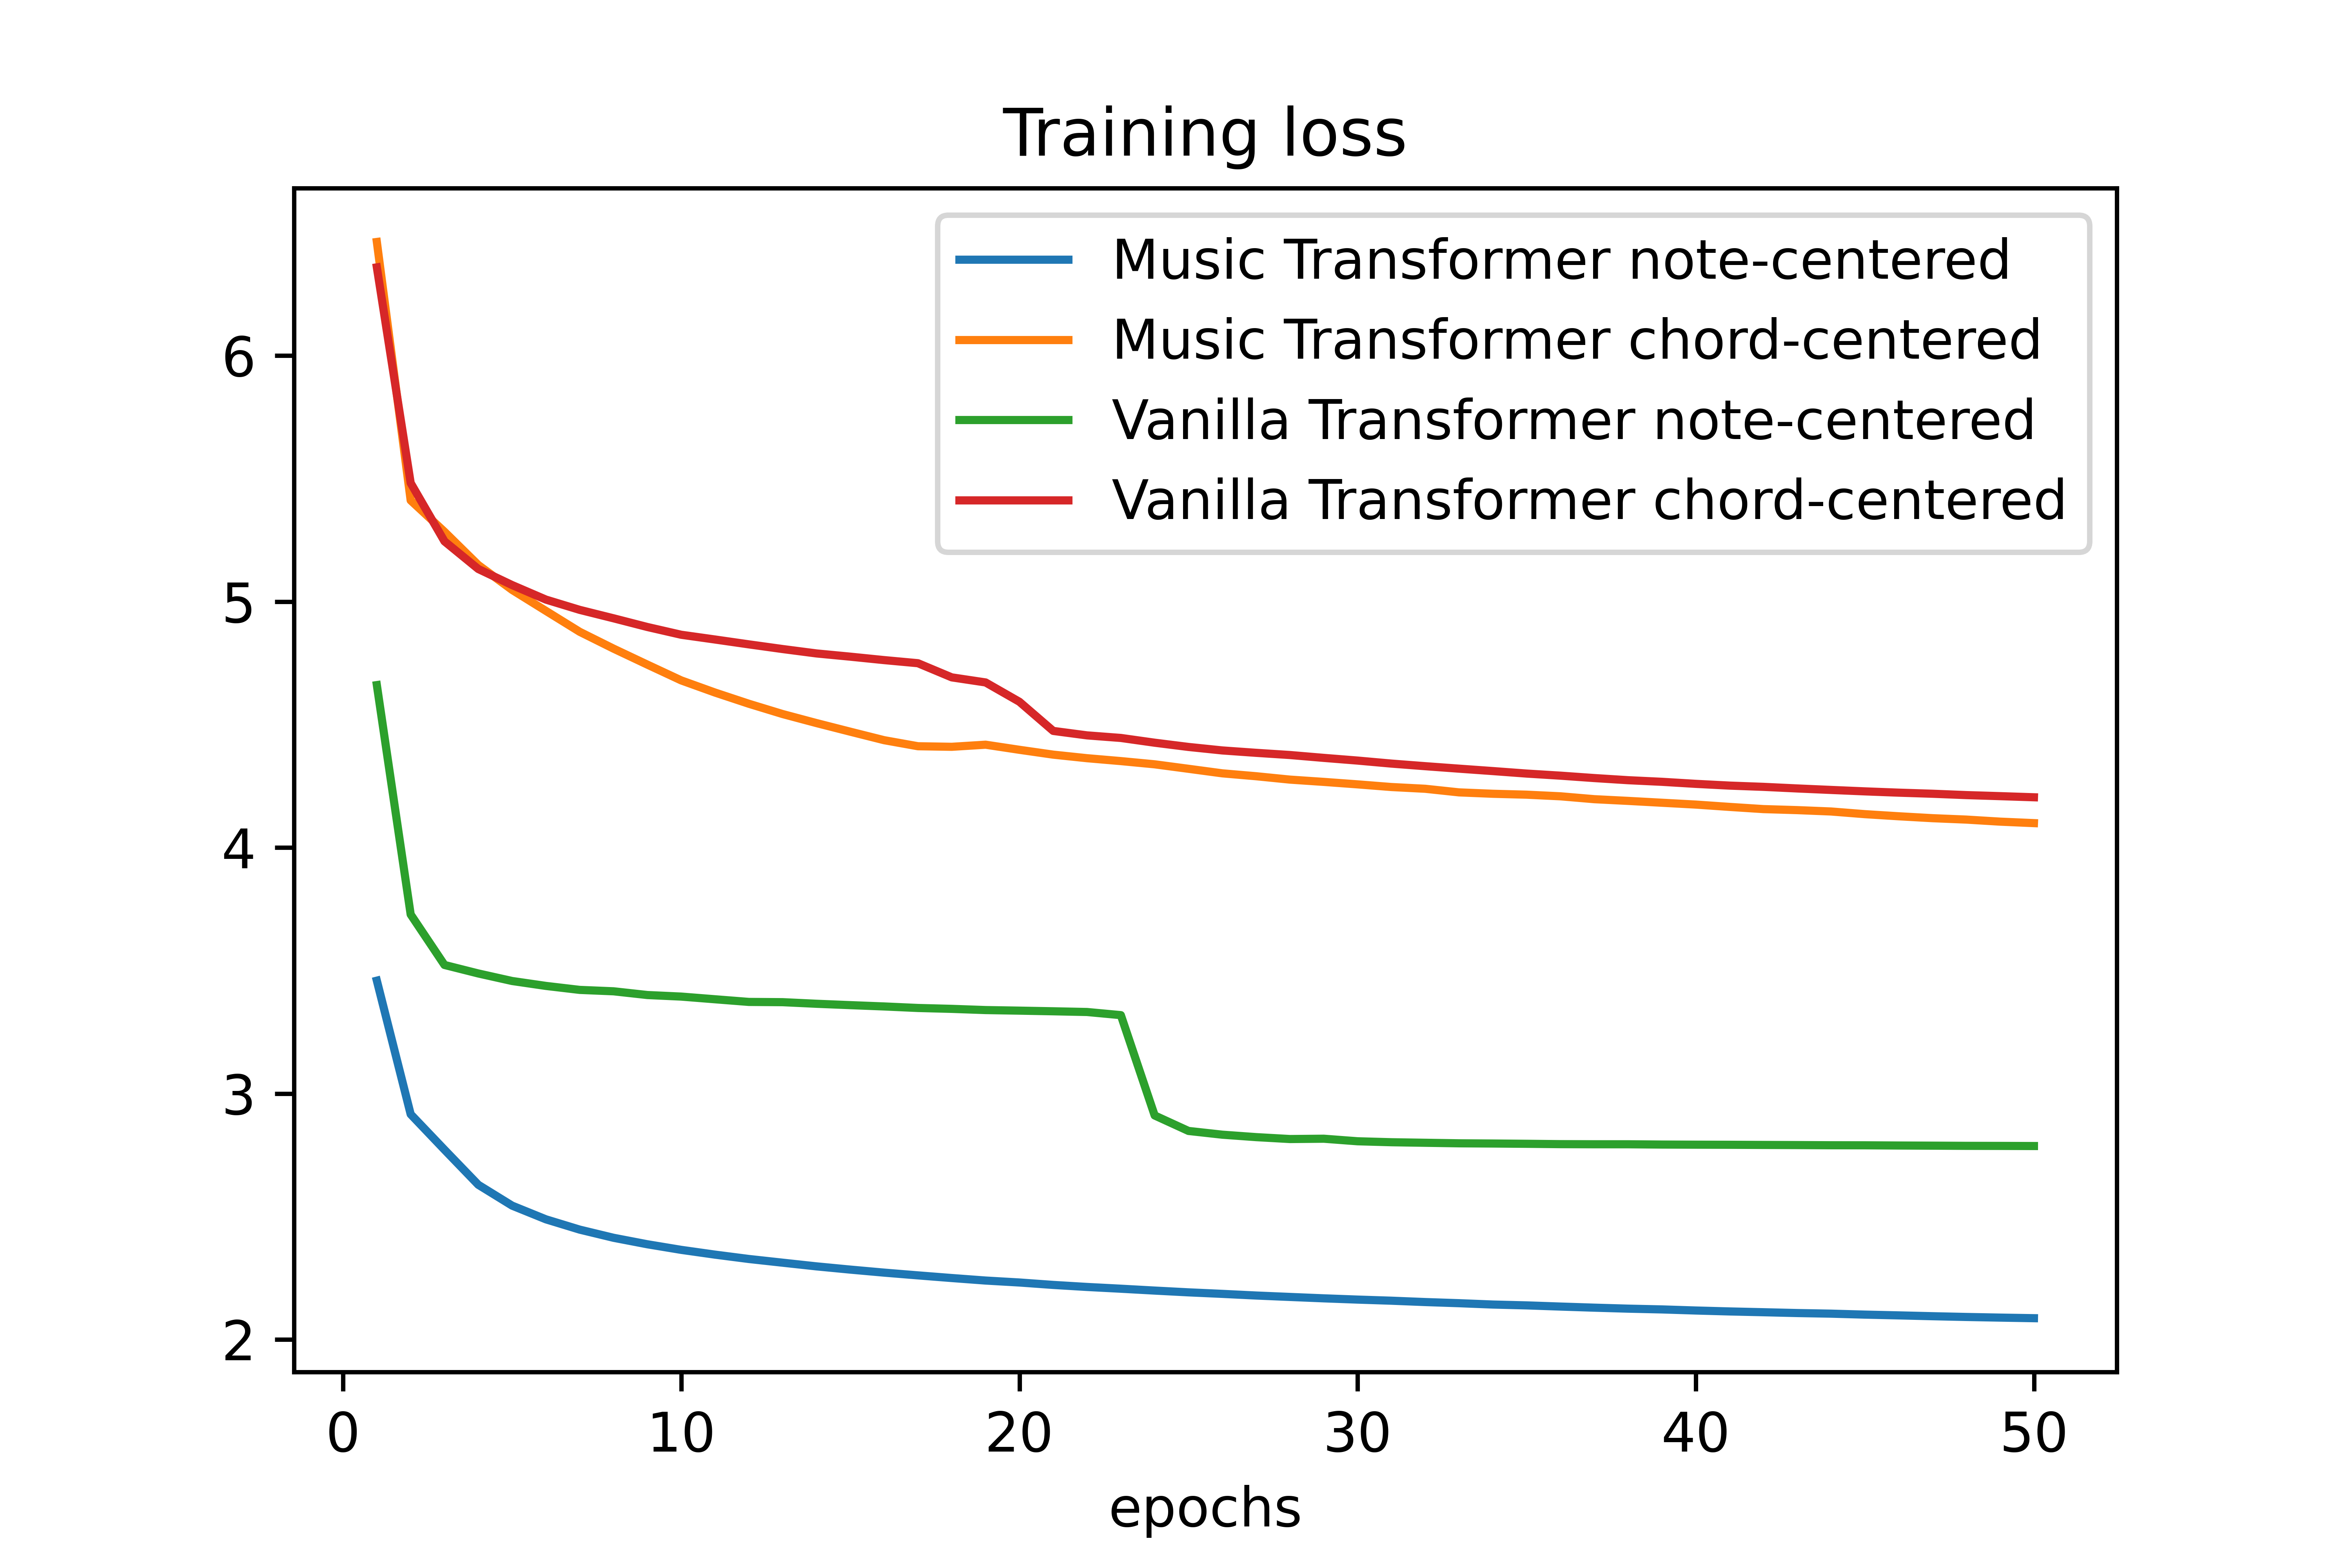
\includegraphics[width=0.8\textwidth]{assets/training-loss}
    \caption{~Loss of models on training set}\label{fig:appendix-training-loss}
\end{figure}
\begin{figure}
    \centering
    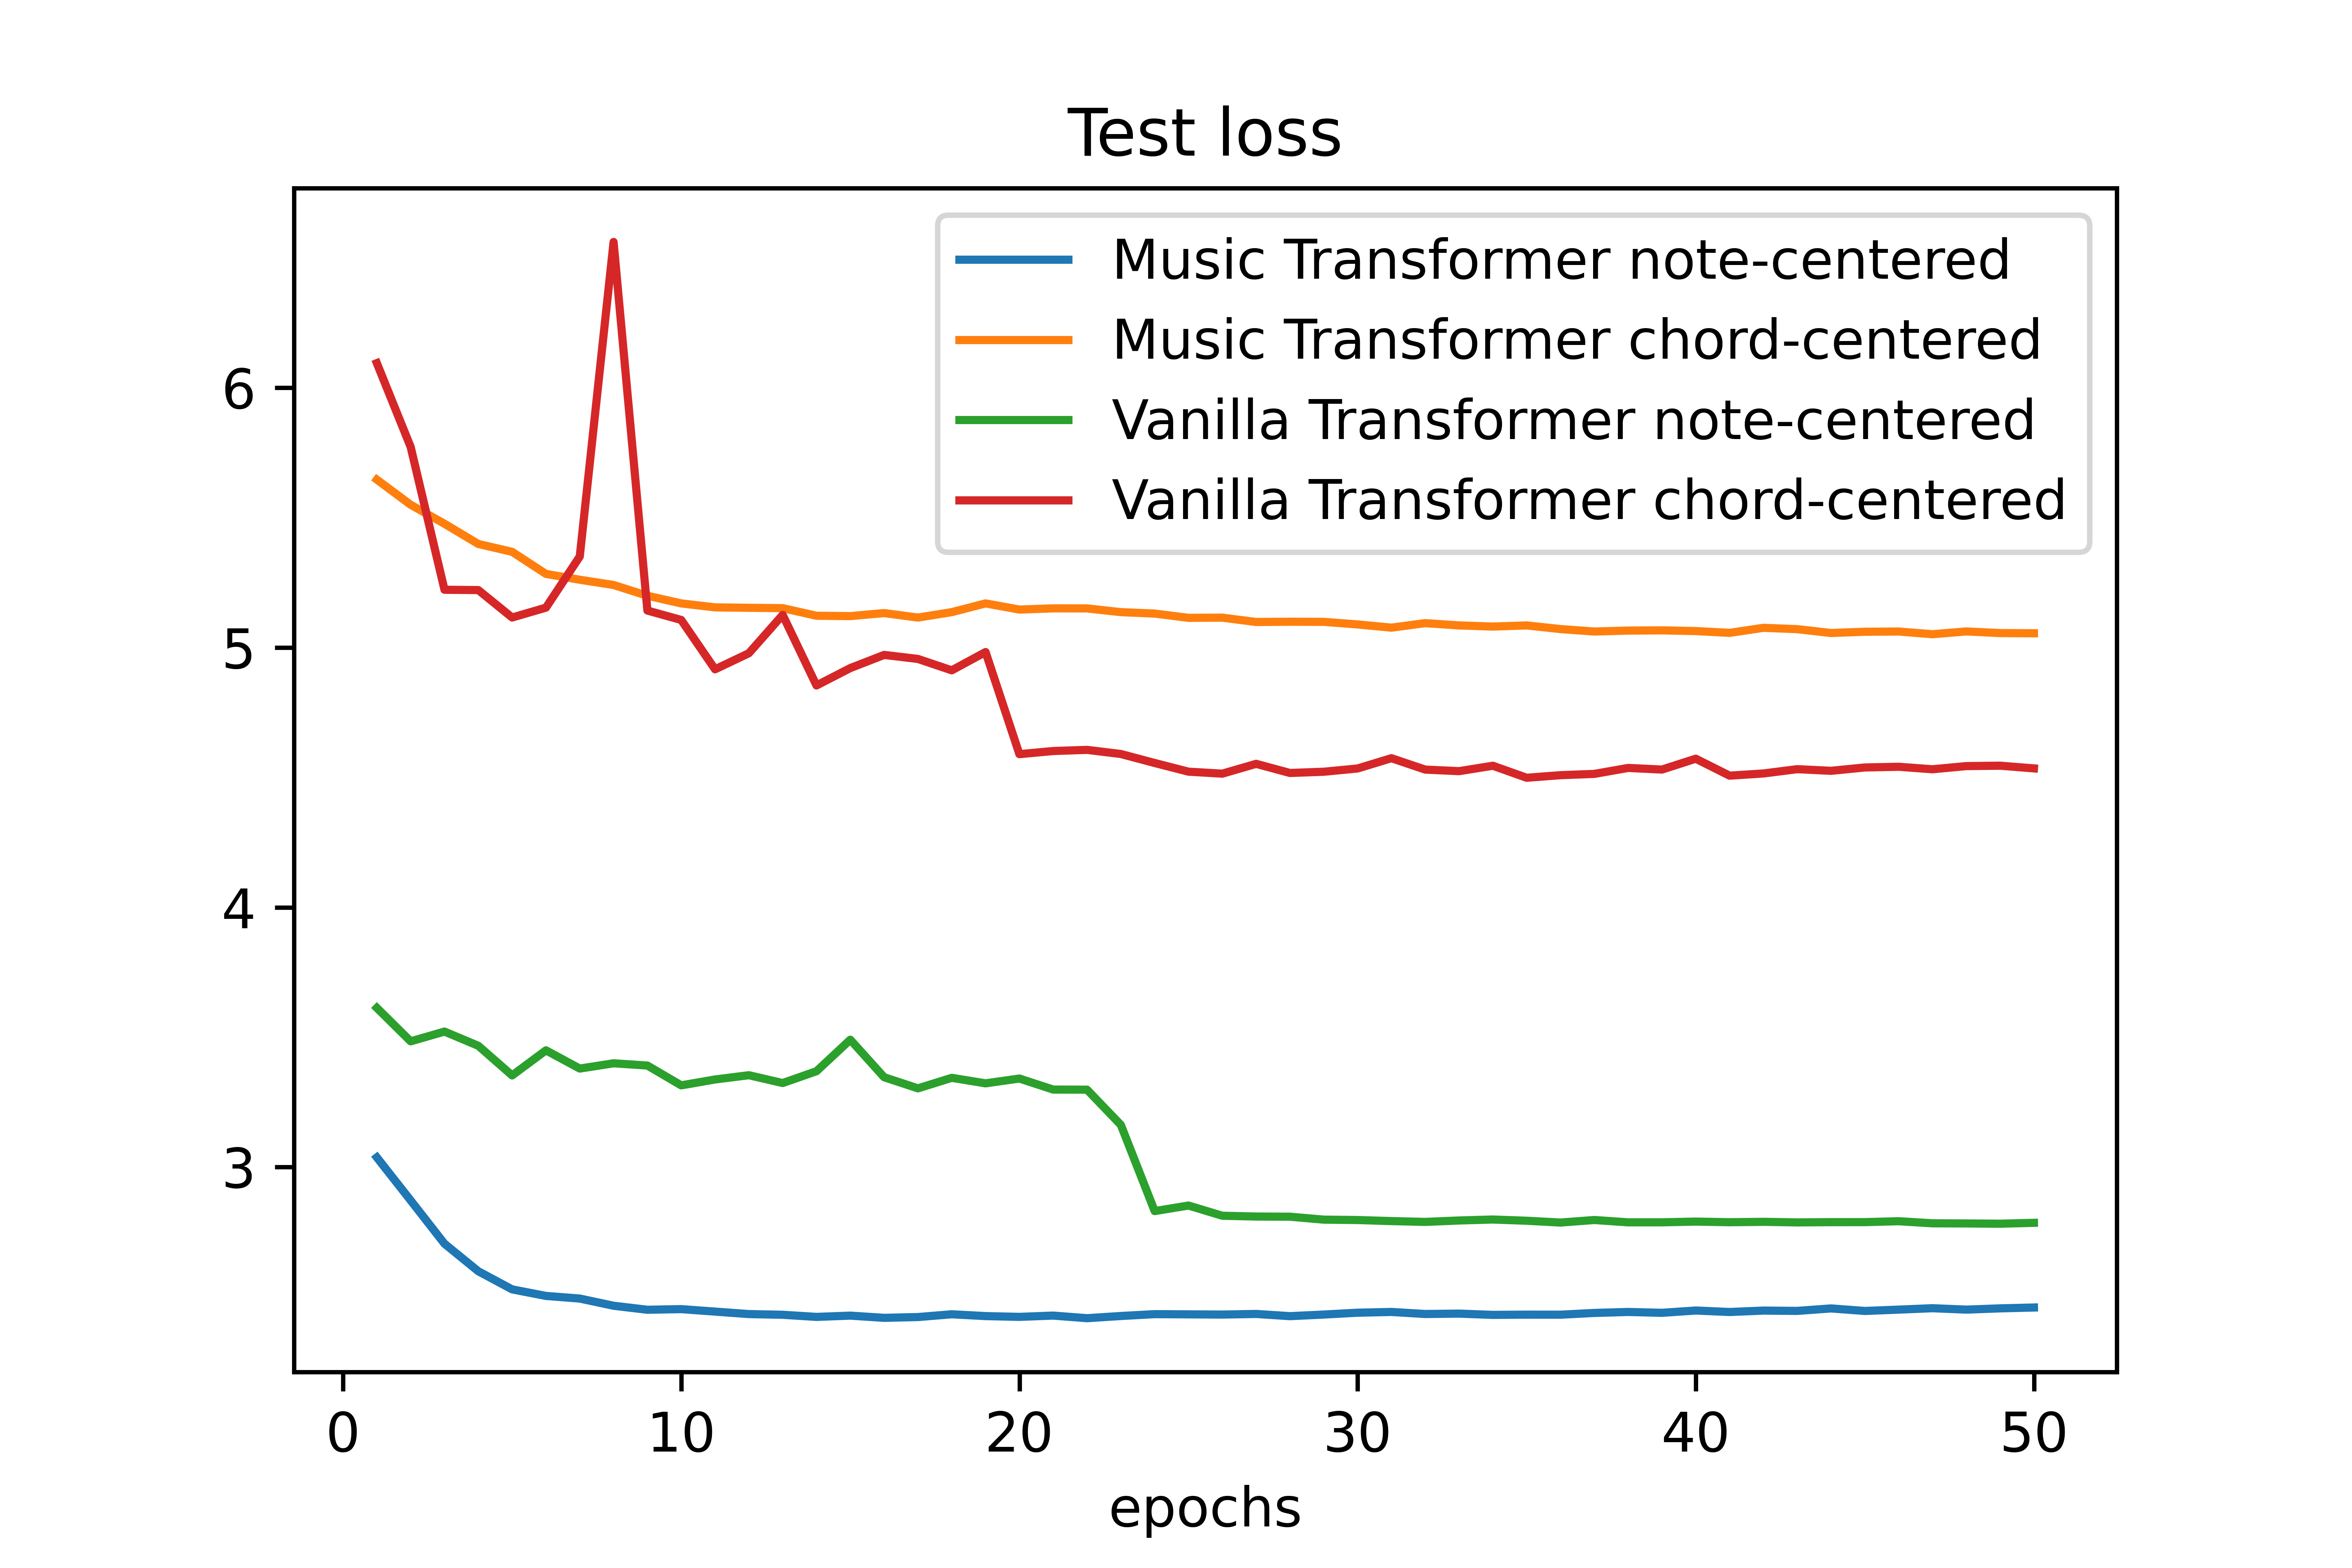
\includegraphics[width=0.8\textwidth]{assets/test-loss}
    \caption{~Loss of models on test set}\label{fig:appendix-test-loss}
\end{figure}

\begin{figure}
    \centering
    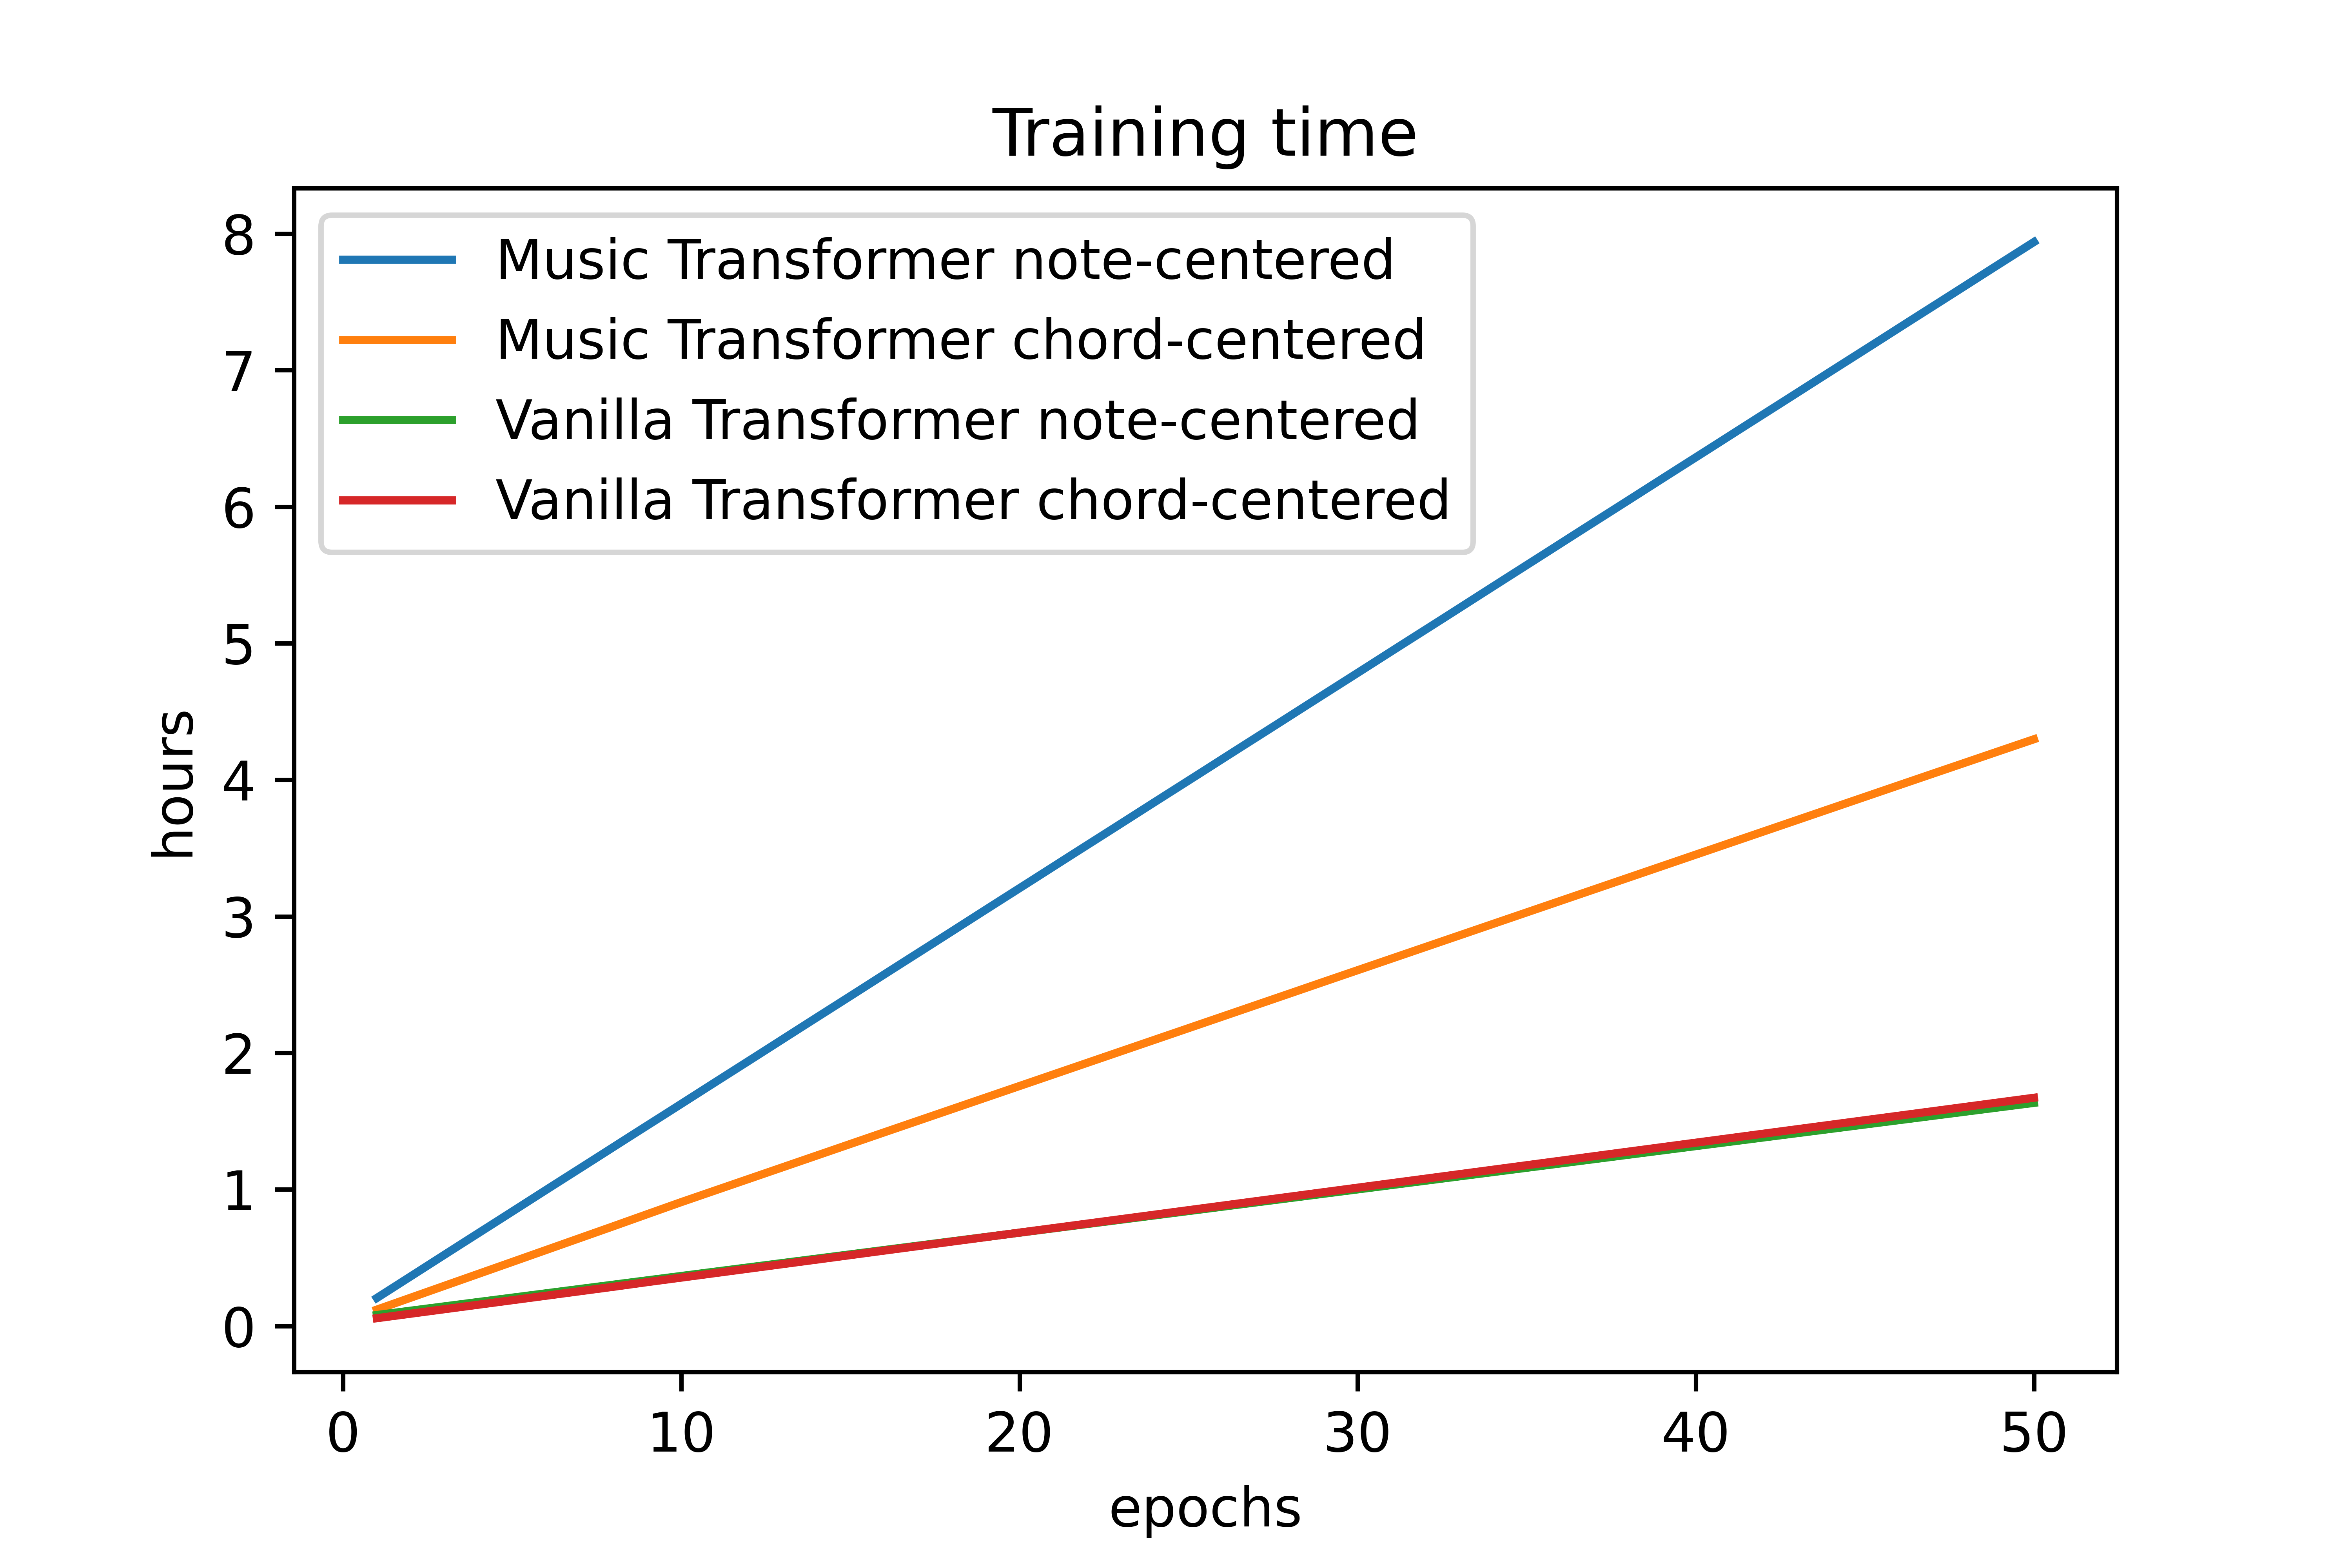
\includegraphics[width=0.8\textwidth]{assets/training-time}
    \caption{~Models training time}\label{fig:appendix-training-time}
\end{figure} % include `appendix.tex' from `text/' subdirectory

    \backmatter % do not remove this command

    \printbibliography % print out the BibLaTeX-generated bibliography list

    \chapter{Contents of attached media}


	\dirtree{%
		.1 src.
		.2 impl\DTcomment{source codes of implementation}.
		.2 thesis\DTcomment{source code format \LaTeX{} of thesis}.
		.2 models\DTcomment{trained models}.
		.1 text\DTcomment{text of the thesis}.
		.2 thesis.pdf\DTcomment{thesis in the PDF format}.
	}
 % include `medium.tex' from `text/' subdirectory

\end{document}
